\documentclass[UTF8,openany,oneside]{ctexbook}

% Shared style for the YouLong AUV technical manual.
\usepackage[a4paper,margin=25mm,headheight=15pt]{geometry}
\usepackage{fontspec}
\usepackage{amsmath,amssymb,mathtools}
\usepackage{booktabs,longtable,tabularx,array,multirow}
\usepackage{graphicx}
\usepackage{xcolor}
\usepackage{tikz}
\usetikzlibrary{arrows.meta,positioning,fit,calc,shapes.geometric}
\usepackage{enumitem}
\usepackage{listings}
\usepackage{siunitx}
\usepackage{fancyhdr}
\usepackage{lastpage}
\usepackage{float}
\usepackage{caption}
\usepackage{mdframed}
\usepackage{needspace}
\usepackage{hyperref}
\usepackage{cleveref}
\usepackage{etoolbox}
\usepackage{biblatex}

\addbibresource{references.bib}

\definecolor{YoulongBlue}{HTML}{145A86}
\definecolor{YoulongDark}{HTML}{17324D}
\definecolor{YoulongLight}{HTML}{EAF3F8}
\definecolor{CodeBackground}{HTML}{F5F7F9}
\definecolor{CodeKeyword}{HTML}{7A1FA2}
\definecolor{CodeComment}{HTML}{4F6B5A}
\definecolor{CodeString}{HTML}{9A3412}
\definecolor{WarningBackground}{HTML}{FFF5E6}
\definecolor{WarningBorder}{HTML}{D97706}

\hypersetup{
  colorlinks=true,
  linkcolor=YoulongBlue,
  citecolor=YoulongBlue,
  urlcolor=YoulongBlue,
  pdftitle={YouLong AUV 系统设计、实现与实验手册},
  pdfauthor={YouLong AUV 控制系统团队}
}

\setlist{topsep=3pt,itemsep=2pt,parsep=2pt}
\setlength{\emergencystretch}{3em}

\sisetup{detect-all=true,per-mode=symbol,range-phrase={--}}

\lstdefinestyle{youlongcode}{
  backgroundcolor=\color{CodeBackground},
  basicstyle=\ttfamily\small,
  keywordstyle=\color{CodeKeyword}\bfseries,
  commentstyle=\color{CodeComment}\itshape,
  stringstyle=\color{CodeString},
  frame=single,
  rulecolor=\color{black!20},
  numbers=left,
  numberstyle=\tiny\color{black!50},
  numbersep=8pt,
  breaklines=true,
  showstringspaces=false,
  columns=fullflexible,
  keepspaces=true,
  tabsize=2
}
\lstset{style=youlongcode}

% URL-style monospaced paths can break at slashes, which keeps interface tables
% readable without manually duplicating line-break decisions in the prose.
% Keep spaces visible in shell commands while allowing path-like macros to
% remain breakable through \topic, \pkg and \pathref below.
\newcommand{\code}[1]{\texttt{\detokenize{#1}}}
\newcommand{\topic}[1]{\path{#1}}
\newcommand{\pkg}[1]{\path{#1}}
\newcommand{\pathref}[1]{\path{#1}}
\newcommand{\repo}{\texttt{YouLong\_AUV\_Control\_System}}
\newcommand{\TODO}[1]{\textcolor{WarningBorder}{[待补充：#1]}}

\newenvironment{infobox}{%
  \begin{quote}\small\color{YoulongDark}%
}{%
  \end{quote}%
}
\newmdenv[
  backgroundcolor=WarningBackground,
  linecolor=WarningBorder,
  linewidth=1pt,
  roundcorner=4pt,
  innerleftmargin=8pt,
  innerrightmargin=8pt,
  innertopmargin=6pt,
  innerbottommargin=6pt,
  skipabove=6pt,
  skipbelow=6pt
]{warningbox}

\newcommand{\statuscurrent}{\textbf{当前实现}}
\newcommand{\statusdesign}{\textbf{设计约束}}
\newcommand{\statusfuture}{\textbf{后续工作}}

\pagestyle{fancy}
\fancyhf{}
\fancyhead[L]{\small\color{YoulongDark}YouLong AUV 系统手册}
\fancyhead[R]{\small\color{YoulongDark}\nouppercase{\leftmark}}
\fancyfoot[C]{\small\thepage\,/\,\pageref{LastPage}}
\renewcommand{\headrulewidth}{0.4pt}
\renewcommand{\footrulewidth}{0pt}

\setcounter{secnumdepth}{3}
\setcounter{tocdepth}{2}

\IfFileExists{build/git-info.tex}{\input{build/git-info.tex}}{}
\providecommand{\DocGitCommit}{unknown}
\providecommand{\DocGitBranch}{unknown}
\providecommand{\DocGitTag}{unknown}
\providecommand{\DocBuildDate}{unknown}

\title{\Huge YouLong AUV 系统设计、实现与实验手册}
\author{YouLong AUV 控制系统团队}
\date{\DocBuildDate}

\begin{document}

\frontmatter
\begin{titlepage}
  \centering
  \vspace*{20mm}
  {\color{YoulongBlue}\rule{\textwidth}{1.5pt}}\\[12mm]
  {\Huge\bfseries YouLong AUV\\[4mm]系统设计、实现与实验手册}\par
  \vspace{12mm}
  {\Large Technical Design, Implementation and Experiment Manual}\par
  \vfill
  \begin{tabular}{ll}
    文档版本 & V1.1（持续维护版）\\
    Git commit & \texttt{\DocGitCommit}\\
    Git 分支 & \texttt{\DocGitBranch}\\
    Git 描述 & \texttt{\DocGitTag}\\
    构建日期 & \texttt{\DocBuildDate}\\
  \end{tabular}
  \vfill
  {\large \today}\par
  \vspace{8mm}
  {\color{YoulongBlue}\rule{\textwidth}{1.5pt}}
\end{titlepage}

\chapter*{文档定位}
\addcontentsline{toc}{chapter}{文档定位}
本手册是 \repo 的正式系统文档。它描述系统的目标、边界、接口、坐标系、
实现现状、实验方法和运维流程。手册不替代代码和参数文件：Topic 名称、消息字段、
标定数值和运行参数仍以仓库中的源码、ROS 接口和配置文件为事实来源。

\begin{infobox}
  阅读时请特别区分“当前实现”和“设计预留”。当前版本的定位后端是 bootstrap
  估计器，规划包是对现有 A* 后端的边界封装；文档会明确标注尚未完成的 FGO、SLAM、
  通用轨迹跟踪等能力。
\end{infobox}

\chapter*{修订记录}
\addcontentsline{toc}{chapter}{修订记录}
\begin{longtable}{p{0.16\textwidth}p{0.20\textwidth}p{0.53\textwidth}}
  \toprule
  版本 & 日期 & 变更摘要 \\
  \midrule
  \endfirsthead
  \toprule
  版本 & 日期 & 变更摘要 \\
  \midrule
  \endhead
  V1.1 & \DocBuildDate & 扩展包级架构、运行时数据流、安全状态模型、构建发布闭环及包/Topic 索引。 \\
  V1.0 & \DocBuildDate & 建立 LaTeX 正式手册；记录双 workspace、/auv 接口、SIL/HIL、定位、视觉、控制、任务与实验边界。 \\
  \bottomrule
\end{longtable}

\chapter*{缩略语}
\addcontentsline{toc}{chapter}{缩略语}
\begin{description}
  \item[AUV] Autonomous Underwater Vehicle，自治水下航行器。
  \item[DVL] Doppler Velocity Log，多普勒测速仪。
  \item[USBL] Ultra-Short Baseline，超短基线定位。
  \item[INS] Inertial Navigation System，惯性导航系统。
  \item[ROS 2] Robot Operating System 2，机器人软件中间件。
  \item[SIL] Software-in-the-Loop，软件在环仿真。
  \item[HIL] Hardware-in-the-Loop，硬件在环仿真。
  \item[MCU] Microcontroller Unit，微控制器。
  \item[NED] North-East-Down，北-东-地坐标约定。
  \item[FRD] Forward-Right-Down，前-右-下机体坐标约定。
  \item[ATE/RPE] Absolute / Relative Trajectory Error，绝对/相对轨迹误差。
\end{description}

\chapter*{阅读指南}
\addcontentsline{toc}{chapter}{阅读指南}
初次接触项目时，建议先读第 1--2 章了解目标和架构，再读第 4--7 章掌握接口、
启动和硬件边界；需要修改算法时阅读第 8--13 章；需要复现实验或下水部署时阅读
第 14--20 章和附录。开发时可同时参考现有 Markdown 快速文档。

\tableofcontents
\listoffigures
\listoftables

\mainmatter
\chapter{项目概述}
\label{ch:overview}

\section{项目定义}
YouLong AUV 是面向水下自主航行、视觉目标识别、目标定位和竞赛任务执行的自治水下航行器软件系统。系统将真实车辆、仿真环境和硬件在环环境统一到一套 ROS 2 接口之后，使任务层和算法层可以在不同运行模式之间迁移。本文档按仓库源码和配置记录当前事实，并以 ROS 2 的节点、Topic、Service、Action 模型作为术语背景 \cite{ros2docs,youlongrepo}。

本项目的核心不是某一个单独算法，而是一条可观测、可替换、可实验的闭环：传感器产生测量，感知和状态估计产生对世界的解释，规划和任务层产生意图，控制层将意图转化为 ZIT6 命令，底层控制核驱动推进器，新的传感器数据再回到估计器。

\section{应用场景}
当前仓库针对 SAUVC/国水等竞赛场景组织任务配置，包含起始、巡游、过门、击球、寻找收集框、抓球、投放以及返回原点等任务模块。任务链位于 \pathref{workspace_auv/src/uv_task/config/missions/}，具体参数位于 \pathref{workspace_auv/src/uv_task/config/tasks/}。

\section{设计目标}
\begin{enumerate}
  \item \textbf{接口一致性：} 真机、SIL 和 HIL 使用相同的传感器、状态、控制和任务接口。
  \item \textbf{状态可信：} 控制、规划和任务只消费估计状态，不消费仿真真值。
  \item \textbf{边界可替换：} 定位器、规划器和感知后端可以在不改变下游接口的情况下替换。
  \item \textbf{可复现实验：} 场景 seed、参数、rosbag、指标和 Git commit 可以绑定在同一次实验中。
  \item \textbf{安全可诊断：} 心跳、watchdog、健康状态、控制频率和传感器退化事件可被记录和检查。
\end{enumerate}

\section{能力边界与当前状态}
\begin{table}[H]
  \centering
  \caption{系统能力的当前实现与边界}
  \label{tab:overview-status}
  \begin{tabularx}{\textwidth}{p{0.25\textwidth}X}
    \toprule
    能力 & 当前状态 \\
    \midrule
    运动执行 & \pkg{uv_control} 提供 BasicMotion Action 和坐标变换，向 ZIT6 输出位置设定值。 \\
    状态估计 & \pkg{uv_localization} 当前实现 bootstrap 估计器；未宣称已实现 FGO、SLAM 或 Active SLAM。 \\
    视觉 & \pkg{uv_camera} 集成相机、YOLO、线检测、ArUco 和目标位置估计。 \\
    规划 & \pkg{uv_nav} 提供 A* 兼容后端；\pkg{uv_planning} 当前主要承担边界封装。 \\
    仿真 & \pkg{stonefish_ros2} 与 \pkg{uv_sim_bridge} 提供 SIL/HIL 链路，Ground Truth 只用于评测。 \\
    \bottomrule
  \end{tabularx}
\end{table}

\section{文档与代码的职责}
代码和配置是机器可执行的事实来源，本手册负责解释其设计意图、数据契约、数学约定和验证方法。对于相机内参、PID 增益、场景坐标和设备路径，手册只记录来源、含义和验证方式，不在正文中维护容易漂移的第二份数值。

\section{术语约定}
除非特别说明，本手册中的“状态”指估计状态，“真值”专指仿真器提供的理想 Ground Truth；“命令”指从上层向控制器或执行器发送的意图；“测量”指传感器或传感器适配器发布的数据。

\chapter{总体系统架构}
\label{ch:architecture}

\section{架构总览}
系统采用 ROS 2 节点化、Topic/Service/Action 解耦的分布式结构。系统启动由 launch 编排，运行时不依赖一个中心控制进程。模块通过 \topic{/auv/...} 交换数据，便于将真实传感器替换为 Stonefish 传感器，或将真实 MCU 替换为 Host 控制核。

\begin{figure}[H]
  \centering
  \begin{tikzpicture}[
    scale=0.82,
    transform shape,
    node distance=8mm and 12mm,
    box/.style={draw=YoulongBlue, rounded corners, fill=YoulongLight,
      minimum width=31mm, minimum height=9mm, align=center},
    io/.style={draw=YoulongDark, rounded corners, fill=white,
      minimum width=34mm, minimum height=9mm, align=center},
    arr/.style={-{Latex[length=2mm]}, thick, color=YoulongBlue}
  ]
    \node[io] (source) {真实传感器\\Stonefish};
    \node[box, right=of source] (adapter) {L1 适配器\\\pkg{uv_hm}/\pkg{uv_sim_bridge}};
    \node[box, right=of adapter] (sensor) {标准传感器\\\topic{/auv/sensors/*}};
    \node[box, below=of sensor] (perception) {感知\\\pkg{uv_camera}};
    \node[box, left=of perception] (localization) {定位\\\pkg{uv_localization}};
    \node[box, below=of localization] (control) {控制\\\pkg{uv_control}};
    \node[box, right=of control] (task) {任务\\\pkg{uv_task}};
    \node[box, right=of task] (actuator) {MCU / 仿真推进器};
    \draw[arr] (source) -- (adapter);
    \draw[arr] (adapter) -- (sensor);
    \draw[arr] (sensor) -- (perception);
    \draw[arr] (sensor) -- (localization);
    \draw[arr] (perception) -- (localization);
    \draw[arr] (localization) -- (control);
    \draw[arr] (task) -- (control);
    \draw[arr] (control) -- (actuator);
    \draw[arr] (actuator.north) |- (source.south);
  \end{tikzpicture}
  \caption{YouLong AUV 的逻辑闭环}
  \label{fig:system-loop}
\end{figure}

\section{双 Workspace 分治}
\pkg{workspace_auv} 包含不依赖 Stonefish 的真机/通用控制栈；\pkg{workspace_sim} 依赖前者并提供 Stonefish、仿真描述、适配器、退化注入和评测。这样，Edge 真机环境可以单独构建控制栈，开发机可以在 overlay 中加入仿真能力。

\begin{table}[H]
  \centering
  \caption{两个工作区的职责}
  \label{tab:workspaces}
  \begin{tabularx}{\textwidth}{p{0.25\textwidth}X}
    \toprule
    工作区 & 主要包与职责 \\
    \midrule
    \pkg{workspace_auv} & 接口、消息、真实 URDF、硬件管理、相机与感知、定位、控制、规划、任务、日志。 \\
    \pkg{workspace_sim} & Stonefish、仿真 URDF、Stonefish 适配器、ZIT6 Host 控制核、传感器退化、评测和 SIL/HIL 启动。 \\
    \bottomrule
  \end{tabularx}
\end{table}

\section{分层与依赖方向}
依赖方向从稳定契约指向实现：\pkg{auv_protocol} 和 \pkg{uv_msgs} 不依赖具体算法；\pkg{uv_perception}、\pkg{uv_planning} 和 \pkg{uv_mapping} 提供接口边界；现阶段具体实现仍在 \pkg{uv_camera} 和 \pkg{uv_nav} 中。运行节点可以订阅多个上游 Topic，但不应跨越接口边界直接访问仿真器内部对象或另一个节点的私有状态。

\section{运行模式}
\begin{description}
  \item[real] 使用真实 URDF、真实相机和真实 ZIT6/MCU 状态；启动入口为 \code{ros2 launch uv_bringup real.launch.py}。
  \item[sim] 使用 Stonefish 和仿真描述，\pkg{uv_sim_bridge} 将仿真输入转换为标准接口；下游控制、感知、规划和任务节点与真机复用。
  \item[hil] 使用仿真世界和真实 ZIT6 控制核/MCU，通过 micro-ROS Agent 传递状态和命令；启动入口为 \code{hil.launch.py}。
\end{description}

\section{关键不变量}
\begin{enumerate}
  \item 固定变换只由 \code{robot_state_publisher} 发布到 \topic{/auv/tf_static}。
  \item 动态 \code{odom -> base_link} 只由 \pkg{uv_localization} 发布到 \topic{/auv/tf}。
  \item \topic{/auv/state/odom} 和 \topic{/auv/state/twist} 是控制、规划、任务允许消费的正式估计状态入口。
  \item \topic{/auv/sim/ground_truth/*} 不进入定位、规划、任务或控制闭环。
  \item 新接口使用 \topic{/auv/...}；无前缀旧接口只出现在兼容桥或旧工具中。
\end{enumerate}

\chapter{机械与硬件平台}
\label{ch:hardware}

\section{平台组成}
车辆硬件由水下舱体、六推进器或等效推进执行机构、前视/下视相机、惯性测量单元、DVL、深度/压力传感器、USBL 接口、MCU 控制器、Jetson/Edge 计算机和电源系统组成。软件通过 \pkg{auv_description} 的 URDF 和组件清单表达车辆几何，通过 \pkg{uv_hm} 和 ZIT6 接口表达控制与状态边界。

\begin{table}[H]
  \centering
  \caption{硬件信息的事实来源}
  \label{tab:hardware-sources}
  \begin{tabularx}{\textwidth}{p{0.31\textwidth}X}
    \toprule
    内容 & 来源与维护方式 \\
    \midrule
    机械尺寸、部件位置、标定参考点 & 项目 \code{docs} 目录中的机械说明 PDF 及 \pkg{auv_description}。 \\
    真实 TF 和传感器安装关系 & \pathref{workspace_auv/src/auv_description/urdf/auv.urdf}。 \\
    真实组件登记 & \pathref{workspace_auv/src/auv_description/config/real_components.yaml}。 \\
    相机内参与立体外参 & \pathref{workspace_auv/src/uv_camera/config/cameras/}、\code{*.npz} 和相机 profile。 \\
    ZIT6 控制参数 & 固件配置和 \pathref{workspace_auv/src/uv_hm/config/}。 \\
    \bottomrule
  \end{tabularx}
\end{table}

\section{推进器与执行器}
SIL 中，ZIT6 控制核输出归一化 6-DOF 机体力/力矩，\pkg{uv_sim_bridge} 的 \code{ThrustMixer} 根据车辆推进器布局完成分配，再通过 \topic{/auv/sim/actuators/thruster_command} 送入 Stonefish。真实系统中，控制核和最终执行器分配可以位于 MCU 或外部电机控制板；上层不应依赖具体的电机编号。

\section{相机平台}
系统将前视和下视相机分别建模为左右目。真实模式中，\pkg{uv_camera} 的传感器线程打开 V4L2 设备并发布标准相机 Topic；仿真模式中，\pkg{uv_sim_bridge} 接收 Stonefish 图像，转发左右目图像并生成时间匹配的 stitched 图像。相机标定的解释和使用见第~\ref{ch:calibration}~章。

\section{计算与通信}
Jetson/Edge 计算机运行 ROS 2 节点、感知和任务；MCU 运行 ZIT6 控制核及底层传感器/执行器接口。HIL 模式通过 micro-ROS Agent 和串口承载 MCU 的 DDS/XRCE 通信。\pkg{workspace_auv} 的真机启动文件不包含 Stonefish，也不强制包含串口 Agent；部署系统应提供可用的 MCU ROS 2 通道。

\section{未测量外参的处理}
当前机械 PDF 没有给出真实 DVL 的安装外参，因此真实 URDF 不发布未经测量的 \code{dvl_link}。收到实测结果后，应先更新组件登记和标定文件，再生成固定 TF；禁止为了“补齐 TF 树”而编造安装位置。

\section{硬件平台待补字段}
以下内容保留为可追溯字段，不能用估计值替代：\TODO{车辆总质量、排水体积、浮力余量、质心/浮心、推进器型号与最大推力、电池容量、MCU 型号、网络地址、完整 pin map 和实物照片}。

\chapter{坐标系、TF、时间与单位}
\label{ch:frames}

\section{坐标系树}
项目采用 ROS 风格的固定/动态变换分工：

\begin{figure}[H]
  \centering
  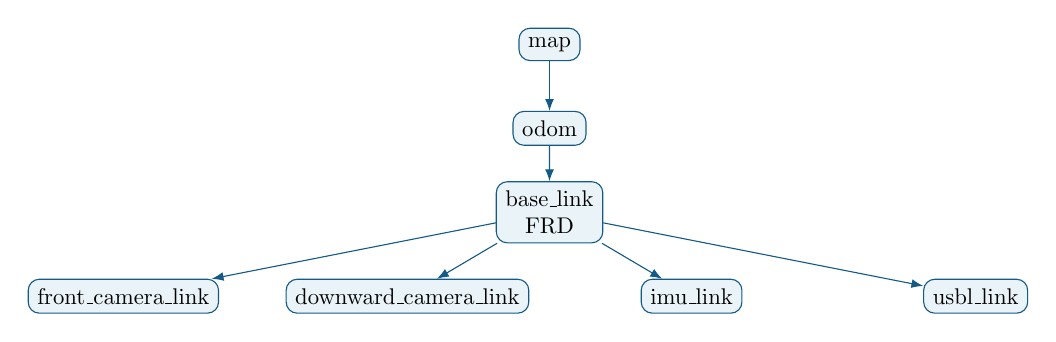
\begin{tikzpicture}[
    level distance=13mm,
    level 3/.style={sibling distance=44mm},
    scale=0.82,
    transform shape,
    every node/.style={draw=YoulongBlue, rounded corners, fill=YoulongLight,
      inner sep=4pt, align=center},
    edge from parent/.style={draw=YoulongBlue, -{Latex[length=1.5mm]}}
  ]
    \node {map}
      child { node {odom}
        child { node {base\_link\\FRD}
          child { node {front\_camera\_link} }
          child { node {downward\_camera\_link} }
          child { node {imu\_link} }
          child { node {usbl\_link} }
        }
      };
  \end{tikzpicture}
  \caption{项目固定和动态 TF 的逻辑树}
  \label{fig:tf-tree}
\end{figure}

\section{世界与机体约定}
世界坐标使用 NED：$x$ 指向北，$y$ 指向东，$z$ 指向下。机体坐标使用 FRD：$x$ 指向前，$y$ 指向右，$z$ 指向下。偏航角零度指向北，顺时针为正。对于仅考虑平面偏航的转换，机体速度到世界速度的关系为
\begin{equation}
  \begin{bmatrix}v_N\\v_E\end{bmatrix}
  =
  \begin{bmatrix}\cos\psi&-\sin\psi\\
  \sin\psi&\cos\psi\end{bmatrix}
  \begin{bmatrix}v_x^b\\v_y^b\end{bmatrix}.
\end{equation}

\section{map、odom 与 body}
\begin{description}
  \item[map] ZIT6 或仿真世界使用的绝对坐标。真实控制命令最终以 map 坐标发送。
  \item[odom] 任务运行时的局部坐标。\code{START} 动作将当前 map 位姿设为 odom 原点，任务通常在该坐标中给出目标。
  \item[body] 以当前车辆位姿为原点的 FRD 机体坐标，用于 BMOVE、BTRAVEL 和机体速度控制。
\end{description}

\section{TF 发布归属}
真实和仿真描述包通过 \code{robot_state_publisher} 发布固定树，并重映射为 \topic{/auv/tf_static}。\pkg{uv_localization} 是动态 \code{odom -> base_link} 的唯一发布者，并输出到 \topic{/auv/tf}。Stonefish Ground Truth 不得成为正式 TF 来源。

\section{单位与兼容字段}
内部算法、canonical 控制设定值和角速度统一使用 SI 单位：位置为 \si{m}，线速度为 \si{m.s^{-1}}，角度为 \si{rad}，角速度为 \si{rad.s^{-1}}。当前 \code{PoseInfo} 为历史兼容消息，其 roll/pitch/yaw 字段仍以度表达；转换只允许出现在消息边界，不能扩散到内部计算。

\section{时间戳}
ROS 消息使用消息 Header 或等价时间字段。仿真模式使用 ROS simulation time，真机模式使用系统/ROS 时间；相机左右目匹配必须依据图像时间戳或 \code{StereoFrameInfo}，禁止将相邻帧简单拼成一个立体对。目标定位还需要用时间最接近的位姿样本补偿车辆运动。

\section{外参命名原则}
每个传感器外参必须说明父坐标系、子坐标系、旋转方向、平移单位和获得方式。相机 optical frame 遵循 ROS 光学坐标约定（$x$ 右、$y$ 下、$z$ 前），不能将图像像素坐标直接当作机体 FRD 坐标。

\begin{warningbox}
坐标系错误通常表现为“控制方向反了”“目标位置随航向旋转错误”或“仿真看起来正确但真机失败”。任何新增传感器、任务或视觉几何代码，都必须在单元测试中给出至少一个轴向和一个偏航旋转的已知答案。
\end{warningbox}

\chapter{ROS 2 软件接口规范}
\label{ch:interfaces}

\section{接口分层}
接口分为三类。\pkg{auv_protocol} 是 Topic/Service/Action 名称的单一注册表；\pkg{uv_msgs} 保存应用层消息、服务和 BasicMotion Action；\pkg{zit6_interfaces} 保存与 ZIT6 固件兼容的设定值、状态和参数服务。新节点应从 \code{auv_protocol.topics} 导入名称，不能在业务代码中散落字符串。

\section{Canonical Topic 空间}
{\small
\begin{longtable}{p{0.29\textwidth}p{0.25\textwidth}p{0.34\textwidth}}
  \caption{主要 Canonical Topic 契约}\label{tab:topics-main}\\
  \toprule
  类别 & Topic 前缀/示例 & 语义 \\
  \midrule
  \endfirsthead
  \toprule
  类别 & Topic 前缀/示例 & 语义 \\
  \midrule
  \endhead
  传感器 & \topic{/auv/sensors/camera/*}, \topic{/auv/sensors/imu/data}, \topic{/auv/sensors/dvl/*} & 真实或仿真适配后的统一测量。 \\
  感知 & \topic{/auv/perception/detections/*}, \topic{/auv/perception/targets} & 检测、线状态、目标观测和目标位置。 \\
  状态 & \topic{/auv/state/odom}, \topic{/auv/state/twist}, \topic{/auv/state/health} & 控制、规划和任务的估计状态入口。 \\
  TF & \topic{/auv/tf}, \topic{/auv/tf_static} & 动态和固定坐标变换。 \\
  控制 & \topic{/auv/basic_motion}, \topic{/auv/control/trajectory} & BasicMotion Action 和规划路径。 \\
  任务 & \topic{/auv/mission/run}, \topic{/auv/mission/status} & Mission 控制服务和状态。 \\
  硬件 & \topic{/auv/hardware/zit6/cmd/*}, \topic{/auv/hardware/zit6/state/*} & ZIT6 下行命令和上行状态。 \\
  仿真 & \topic{/auv/sim/raw/*}, \topic{/auv/sim/ground_truth/*}, \topic{/auv/sim/actuators/*} & 仿真原始输入、真值和执行器接口。 \\
  \bottomrule
\end{longtable}
}

\Needspace{6\baselineskip}
\section{状态接口现状}
\topic{/auv/state/odom} 当前实际消息类型是 \path{uv_msgs/PoseInfo}，而不是最终形态的 \path{nav_msgs/Odometry} 或 \path{uv_msgs/AuvState}。这是有意保留的兼容边界：\code{PoseInfo} 的 yaw 字段为度，\pkg{uv_localization} 内部仍使用弧度。未来更换状态消息时，应保持 Topic 语义稳定，并在迁移期提供明确的转换器。

\section{QoS 与有效性}
高频图像采用只保留最新样本的 Best Effort 策略，避免 CPU/IO 短暂阻塞导致处理旧帧；状态和控制消息使用可靠的普通队列策略，具体深度由启动代码和节点设置。任何消息契约必须同时说明：消息类型、发布者、订阅者、频率、时间戳来源、frame id、单位、有效条件、超时行为和是否允许为空。

\section{Service 与 Action}
\begin{table}[H]
  \centering
  \caption{当前主要 Service/Action}
  \label{tab:services-actions}
  \begin{tabularx}{\textwidth}{p{0.28\textwidth}p{0.24\textwidth}X}
    \toprule
    名称 & 类型 & 用途 \\
    \midrule
    \topic{/auv/basic_motion} & \code{uv_msgs/BasicMotion} Action & SET、WMOVE、BMOVE、WTRAVEL、BTRAVEL、START。 \\
    \topic{/auv/mission/run} & \code{uv_msgs/RunTask} & 启动任务或任务链。 \\
    \topic{/auv/mission/stop} & \code{std_srvs/Trigger} & 停止当前任务。 \\
    \topic{/auv/mission/execute} & \code{uv_msgs/ExecTask} & 调试执行单个任务。 \\
    \topic{/auv/planning/navigate_to} & \code{uv_msgs/RunTask} & 请求 A* 规划。 \\
    \bottomrule
  \end{tabularx}
\end{table}

\section{兼容接口}
旧的 \topic{/task/*}、\topic{/basic_motion*} 和 \topic{/zit6/*} 只应由兼容适配器暴露。当前若干节点仍同时发布新旧 Topic，以便已有 Foxy 固件和调试工具过渡；新业务代码不得依赖旧名字。

\Needspace{7\baselineskip}
\section{接口变更流程}
新增字段优先保持向后兼容；改变单位、frame 或语义时必须提升协议版本，更新 \pathref{docs/architecture/} 下的契约、相关测试和本手册，并在实验记录中绑定 commit。不能只修改 LaTeX 表格而不修改生成消息或 Topic 注册表。

\chapter{Bringup 与配置系统}
\label{ch:bringup}

\section{启动组织}
启动文件只负责编排节点、声明参数、选择 profile、建立 remap 和处理关键进程退出；算法状态和业务逻辑留在节点实现中。真机启动由 \pkg{uv_bringup} 管理，仿真启动由 \pkg{uv_sim_bringup} 管理。

\begin{figure}[H]
  \centering
  \begin{tikzpicture}[
    box/.style={draw=YoulongBlue, rounded corners, fill=YoulongLight,
      minimum width=34mm, minimum height=8mm, align=center},
    arr/.style={-{Latex[length=2mm]}, thick, color=YoulongBlue},
    node distance=7mm
  ]
    \node[box] (real) {\code{real.launch.py}};
    \node[box, below left=of real] (desc) {真实 URDF};
    \node[box, below=of real] (hw) {\pkg{uv_hm}};
    \node[box, below right=of real] (loc) {\pkg{uv_localization}};
    \node[box, below=of hw] (ctrl) {控制 / 感知 / 规划 / 任务};
    \draw[arr] (real) -- (desc);
    \draw[arr] (real) -- (hw);
    \draw[arr] (real) -- (loc);
    \draw[arr] (desc) |- (ctrl);
    \draw[arr] (hw) -- (ctrl);
    \draw[arr] (loc) -- (ctrl);
  \end{tikzpicture}
  \caption{真机 bringup 组成}
  \label{fig:real-bringup}
\end{figure}

仿真入口 \code{sim.launch.py} 额外启动仿真 URDF、Stonefish、\pkg{uv_sim_bridge}、可选退化节点、评测和观测工具；HIL 入口再启动 micro-ROS Agent 并将 \code{hil_mode} 传给 bridge。

\section{Profile 机制}
profile 是标准 ROS 2 YAML 参数文件，用于按模式选择保守或开发参数。当前可见 profile 包括：
\begin{itemize}
  \item real：\code{real_default}、\code{real_safe}；
  \item sim：\code{sim_dev}、\code{sim_ci}；公开 \pkg{uv_sim} 入口另提供
        \code{guoshui}、\code{guoshui_cruise}、\code{guoshui_cruise_seeded}、
        \code{sauvc_finals} 和 \code{sauvc_qualification} world 预设；
  \item hil：\code{hil_lab}。
\end{itemize}
启动文件在进入子 launch 前解析 profile 路径并校验 profile 与运行模式匹配，避免将仿真参数误用于真机。

\Needspace{12\baselineskip}
\section{常用启动命令}
\begin{lstlisting}[language=bash,caption={标准运行入口}]
# Real
cd workspace_auv
colcon build --symlink-install
source install/setup.bash
ros2 launch uv_bringup real.launch.py profile:=real_default

# SIL
cd workspace_sim
colcon build
source install/setup.bash
ros2 launch uv_sim_bringup sim.launch.py profile:=sim_dev

# 公开场景预设；显式 world:= 会覆盖预设 world
ros2 launch uv_sim sim.launch.py profile:=sauvc_finals

# HIL
ros2 launch uv_sim_bringup hil.launch.py profile:=hil_lab \
  serial_dev:=/dev/ttyUSB0 serial_baud:=921600
\end{lstlisting}

\section{启动顺序与就绪}
典型依赖顺序是：描述/固定 TF、硬件或仿真输入、定位、控制、相机/感知、规划、任务。任务默认关闭，避免节点刚启动时立即执行 Mission。\pkg{uv_bringup} 提供 readiness 检查，可按 backend、control、sensors、perception 阶段确认 Topic 和节点已达到运行条件。

\section{参数事实来源}
启动参数的默认值在 launch 中定义，模式参数在 profile 中覆盖，任务参数在 Mission/Task YAML 中维护，相机参数在相机 profile 和标定文件中维护。参数优先级和最终生效值应通过启动日志或 ROS 参数查询确认；LaTeX 不复制完整参数树，附录只列出入口和语义。

\chapter{Hardware Manager 与底层通信}
\label{ch:hardware-manager}

\section{边界职责}
\pkg{uv_hm} 是 ROS 侧的硬件管理节点，当前职责包括：以固定频率发送心跳/布防命令；订阅 ZIT6 状态、心跳和推进器状态；执行电池、错误标志、通信超时和推力饱和监控；将已有旧 \topic{/zit6/state/*} 数据适配到 \topic{/auv/hardware/zit6/state/*}。

它不是一个把所有底层设备细节都塞进来的“大硬件类”。真实 MCU 的固件控制核、传感器驱动和串口传输属于 MCU/外部 micro-ROS 通道；ROS 节点只依赖稳定的 ZIT6 Topic/Service 边界。

\section{ZIT6 命令与状态}
\begin{table}[H]
  \centering
  \caption{ZIT6 Canonical 接口}
  \label{tab:zit6-interface}
  \begin{tabularx}{\textwidth}{p{0.37\textwidth}p{0.24\textwidth}X}
    \toprule
    Topic/Service & 类型 & 语义 \\
    \midrule
    \topic{/auv/hardware/zit6/cmd/setpoint} & \code{ZitSetpoint} & 位置、速度或力设定值。 \\
    \topic{/auv/hardware/zit6/cmd/heartbeat} & \code{UInt32} & 心跳和布防模式。 \\
    \topic{/auv/hardware/zit6/cmd/ins} & \code{UInt8} & INS/DVL 控制。 \\
    \topic{/auv/hardware/zit6/cmd/light}、\code{/servo} & 基础标量消息 & 灯光和舵机设备命令。 \\
    \topic{/auv/hardware/zit6/state/status} & \code{ZitStatus} & 布防、INS、控制级别、电池和错误状态。 \\
    \topic{/auv/hardware/zit6/state/position} & \code{Float32MultiArray} & 兼容的原始位置状态。 \\
    \topic{/auv/hardware/zit6/state/velocity} & \code{Float32MultiArray} & 兼容的原始速度状态。 \\
    \topic{/auv/hardware/zit6/get_params}、\code{/update_params} & ZIT6 Service & PID/控制参数在线查询和更新。 \\
    \bottomrule
  \end{tabularx}
\end{table}

\section{心跳与 watchdog}
心跳发送器按 profile 选择的频率发布命令；硬件管理器记录 MCU 上行心跳和状态最后到达时间。超过 watchdog 阈值时进入 degraded 记录并发出错误日志。电池低于阈值、状态错误标志非零或推进器接近饱和时，系统应进入人工检查流程，而不是继续假设车辆健康。

\section{SIL 中的等价边界}
SIL 的 \pkg{uv_sim_bridge} 模拟 ZIT6 的 Topic/Service 行为，使用 \pkg{zit6_control_core} 的 Host 控制核产生 6-DOF 力，再用推进器 mixer 连接 Stonefish。这样控制、任务和状态消费方看到的接口与真机一致，而底层执行介质不同。

\section{HIL 通信}
HIL 中，micro-ROS Agent 通过串口连接真实 MCU。这里的 Agent 边界遵循 micro-ROS 的典型部署方式 \cite{micro_ros}。仿真侧 bridge 将标准仿真传感器数据交给状态估计，并将估计状态作为 MCU 导航输入；MCU 输出的控制/推力状态经过 bridge 的执行器适配后驱动 Stonefish。Ground Truth 不作为 MCU 的导航输入。

\section{安全原则}
\begin{enumerate}
  \item 未收到有效状态或导航未就绪时，位置/速度设定值不能被当成有效闭环。
  \item heartbeat 丢失、MCU 异常解锁或通信超时时必须可观测并停止继续扩展运动命令。
  \item 任何强制布防模式只允许在明确的实验/维护 profile 中启用。
  \item 在线更新 PID 后必须记录参数快照、时间和 Git commit。
\end{enumerate}

\chapter{状态估计与定位}
\label{ch:localization}

\section{状态边界}
\pkg{uv_localization} 是正式状态发布者。其输出为：估计位姿 \topic{/auv/state/odom}、机体速度 \topic{/auv/state/twist}、健康状态 \topic{/auv/state/health} 和动态 TF \topic{/auv/tf}。控制、规划和任务只应从这些 Topic 获取当前车辆状态。

\section{当前 bootstrap 实现}
当前估计器在真机模式下读取 ZIT6 原始位置/速度，并根据启动或 START 建立 odom 原点；在仿真/HIL 模式下读取 canonical DVL、IMU 和可用性信息，以简单航位推算积分状态。实现刻意不订阅 \topic{/auv/sim/ground_truth/odom}。该边界允许未来把内部实现替换成 FGO/ESKF/SLAM，而不改下游 Topic。

\section{状态表示}
用于设计讨论的连续状态可以写成
\begin{equation}
  \mathbf{x} = \begin{bmatrix}
    \mathbf{p}^{n} & \mathbf{v}^{b} & \boldsymbol{\theta}^{n} &
    \mathbf{b}_{g} & \mathbf{b}_{a}
  \end{bmatrix}^{\mathsf T},
\end{equation}
其中 $\mathbf{p}^{n}$ 是 NED 位置，$\mathbf{v}^{b}$ 是 FRD 机体速度，$\boldsymbol{\theta}^{n}$ 是姿态参数，$\mathbf{b}_{g}$ 和 $\mathbf{b}_{a}$ 分别为陀螺和加速度计偏置。当前实现只使用其中一部分字段，并不代表所有状态量已经被估计。

\section{传感器使用}
\begin{description}
  \item[DVL] 提供机体线速度；无效、非有限或超时数据不应更新估计状态。
  \item[IMU] 当前 bootstrap 实现使用角速度，姿态融合和偏置估计留给后续估计器。
  \item[USBL] 当前边界记录有效性供健康/后续融合使用，不宣称已经完成全量融合。
  \item[压力计] 提供深度相关观测，具体使用方式应由后续状态估计实现明确规定。
\end{description}

\section{原点与 reset}
\topic{/auv/state/reset} 用于重新建立 odom 原点。\code{START} 动作由 \pkg{uv_control} 发布 reset 请求；估计器记录当前原始位置为新原点，之后将局部位置和 yaw 归零。重新定义原点时，控制器的动作目标也必须同步清零。

\section{健康状态}
健康消息至少应包含传感器/估计器名称、可用标志、质量分数、时间戳和人类可读的 detail。健康状态用于 readiness、评测和故障诊断，但不能被误认为是一个具有统计意义的完整协方差。

\section{未来定位后端接口}
未来 FGO、ESKF 或 SLAM 后端必须满足：继续发布相同的估计状态 Topic；明确状态坐标系和时间基准；提供协方差或质量含义；可处理 DVL 丢失、USBL 离群、视觉间歇观测和时间延迟；不得订阅仿真真值。算法替换应通过同一包内的实现选择或插件边界完成。

\begin{warningbox}
当前的 bootstrap 估计器适合接口打通、SIL/HIL 回归和控制链路验证，不应在实验报告中写成高精度融合定位系统。若需要发表定位精度结果，必须说明传感器组合、估计器版本、真值对齐方法和数据集来源。
\end{warningbox}


\chapter{视觉感知与目标定位}
\label{ch:perception}

\section{处理链}
\pkg{uv_camera} 当前将传感器和 AI 组合在同一个 ROS 进程中。传感器模块从真实 V4L2 或仿真 stitched Topic 获取 BGR 帧，通过内存中的 FrameGate 交给 AI 模块；AI 模块执行 YOLO 检测、线状态提取、ArUco 检测、可选数据集记录和标注视频缓存。传感器到 AI 之间不再经过 ROS 图像 Topic 或中间 JPEG 编码。

\begin{figure}[H]
  \centering
  \begin{tikzpicture}[
    node distance=7mm and 10mm,
    box/.style={draw=YoulongBlue, rounded corners, fill=YoulongLight,
      minimum width=30mm, minimum height=9mm, align=center},
    arr/.style={-{Latex[length=2mm]}, thick, color=YoulongBlue}
  ]
    \node[box] (src) {V4L2 / Stonefish\\图像源};
    \node[box, right=of src] (gate) {FrameGate\\BGR 内存帧};
    \node[box, right=of gate] (yolo) {YOLO\\检测/分割};
    \node[box, below=of yolo] (line) {线/ArUco\\辅助检测};
    \node[box, left=of line] (det) {DetectionArray\\按左右目发布};
    \node[box, left=of det] (loc) {object\_localizer\\几何与跟踪};
    \draw[arr] (src) -- (gate) -- (yolo);
    \draw[arr] (yolo) -- (det);
    \draw[arr] (yolo) -- (line);
    \draw[arr] (det) -- (loc);
    \draw[arr] (line) |- (loc);
  \end{tikzpicture}
  \caption{视觉感知与目标定位链路}
  \label{fig:perception-pipeline}
\end{figure}

\section{感知接口}
AI 对每个相机左右目发布 \code{DetectionArray}，包括类别、置信度、bbox、帧时间和 stereo pair id；同时发布线状态和 ArUco ID。目标定位节点订阅四个相机通道和 \topic{/auv/state/odom}，发布：
\begin{itemize}
  \item \topic{/auv/perception/observations}：最近的几何有效观测；
  \item \topic{/auv/perception/targets}：按目标类别/实例维护的静态位置估计；
  \item 兼容的 \code{ObjectPositionArray}：供当前任务和导航后端使用。
\end{itemize}

\section{三类几何观测}
当前目标定位将观测形式显式区分为：前视双目直接三维点、前视多视角射线以及下视已知高度直接测量。对一条相机射线，像素去畸变并转换到机体坐标后，可写为
\begin{equation}
  \mathbf{r}^{n}(\lambda) = \mathbf{p}_{c}^{n} + \lambda\,\mathbf{d}^{n},
  \qquad \lambda>0,
\end{equation}
其中 $\mathbf{p}_{c}^{n}$ 是相机中心，$\mathbf{d}^{n}$ 是在 odom/NED 中归一化的方向。两条不完全相交的射线使用最短连线中点作为候选点，并根据夹角、残差、边缘裁剪和时间一致性判断是否接受。

\section{关联与实例}
目标类别 ID、类别别名和物理类别需要分开：检测器输出保留原始类别，前视/下视别名可以绑定到同一个物理类别，但前视和下视估计可以独立保留，避免一次错误关联污染另一套估计。相同类别的多个目标通过实例 ID、空间距离、观测历史和支持数量进行管理；超过实例上限或几何约束失败的观测必须计数并丢弃。

\section{误差与置信度}
目标位置输出携带 $3\times3$ 协方差和观测形式计数。双目深度误差会随视差减小而快速增大，因此目标定位不应只依赖 bbox 置信度；应同时考虑视差、极线误差、bbox 是否贴边、姿态时间对齐、射线夹角和历史支持。置信度是工程质量分数，不能直接当作概率。

\section{失败情况}
相机无帧、左右目不同步、标定缺失、bbox 贴边、类别不一致、极线误差过大、射线近平行、目标过期和姿态过期都应有可观测的拒绝原因。视觉节点可以发布空检测结果以维持数据流和 readiness，但不能把“没有模型”伪装成“没有目标”。

\section{模型和标定文件}
模型权重与类别映射位于 \pathref{workspace_auv/src/uv_camera/weights/}，相机 profile 与 \code{*.npz} 位于 \pathref{workspace_auv/src/uv_camera/config/}。权重、内参和外参不应复制进 LaTeX；本手册只记录版本、来源、坐标转换和验证结果。


\chapter{导航与规划}
\label{ch:navigation}

\section{当前结构}
\pkg{uv_planning} 是规划边界包，当前启动时实际调用 \pkg{uv_nav} 的 \code{navigator} 节点。\pkg{uv_nav} 读取估计状态和感知得到的目标/障碍位置，使用 \code{AStarPlanner} 生成当前阶段的 WaypointPath，并通过 \topic{/auv/control/trajectory} 发布。

\section{A* 规划}
当前二维 A* 将平面离散为给定分辨率的栅格，使用障碍物安全半径检查候选点和线段。规划输入至少包括起点、目标点、障碍位置和安全半径；输出为一组带深度、航向和速度字段的 \code{Waypoint}。若目标不可达，应返回明确失败原因，不应返回静默的空路径。

\section{服务接口}
\topic{/auv/planning/navigate_to} 接收以字符串编码的目标参数，当前兼容格式为 \code{x,y} 或 \code{x,y,z}。服务成功表示“规划成功并发布路径”，不等价于车辆已经到达目标。

\section{规划与执行的边界}
当前 navigator 的实现主要发布路径并记录导航信息；它不直接调用 BasicMotion Action，也没有通用的轨迹跟踪器消费全部 WaypointPath。现阶段竞赛任务通常由 \pkg{uv_task} 直接调用 \pkg{uv_control} 执行 SET/WMOVE/BMOVE/TRAVEL。未来若接入路径跟踪器，应新增清晰的路径跟踪节点或 Action，不能让 planner 隐式地控制车辆。

\begin{table}[H]
  \centering
  \caption{规划数据流}
  \label{tab:planning-flow}
  \begin{tabularx}{\textwidth}{p{0.27\textwidth}p{0.30\textwidth}X}
    \toprule
    输入 & 处理 & 输出 \\
    \midrule
    \topic{/auv/state/odom} & 读取当前起点和深度/航向 & Waypoint 起点 \\
    \topic{/auv/perception/observations} & 形成障碍物集合 & 栅格占用约束 \\
    navigate service 目标 & A* 搜索与安全半径检查 & \topic{/auv/control/trajectory} \\
    \bottomrule
  \end{tabularx}
\end{table}

\section{后续规划能力}
完整规划层应逐步补齐局部/全局规划、路径跟踪、在线重规划、动态障碍、控制可达性、深度约束和任务优先级。每项能力都必须保持只消费估计状态和标准感知结果，不得读取仿真真值。


\chapter{运动控制}
\label{ch:control}

\section{控制层职责}
\pkg{uv_control} 的核心节点是 \code{basic_motion}。它提供面向任务的 BasicMotion Action，维护 odom/map/body 坐标转换，按动作类型生成目标位姿，并将唯一的底层协议出口收敛到 ZIT6 Setpoint。控制节点消费 \topic{/auv/state/odom}、\topic{/auv/state/twist} 和 ZIT6 状态。

\section{动作类型}
\begin{description}
  \item[SET] 在 odom 中设置绝对目标；未指定轴由调用方或控制器保持。
  \item[WMOVE] 在世界/NED 坐标中按增量移动。
  \item[BMOVE] 在当前 FRD 机体坐标中按增量移动，再转换到 odom/map。
  \item[WTRAVEL/BTRAVEL] 沿直线目标方向移动，适合过门、巡线等任务。
  \item[START] 记录当前位置为 odom 原点，并发送状态 reset。
\end{description}

\section{坐标转换}
控制接口的高层目标通常使用 odom 坐标；ZIT6 协议出口使用 map 坐标。以 yaw 为例，若 odom 原点在 map 中的位姿为 $(x_o,y_o,\psi_o)$，则局部点到 map 的变换为
\begin{equation}
  \begin{bmatrix}x_m\\y_m\end{bmatrix}
  = \begin{bmatrix}x_o\\y_o\end{bmatrix}
  + \begin{bmatrix}\cos\psi_o&-\sin\psi_o\\
  \sin\psi_o&\cos\psi_o\end{bmatrix}
  \begin{bmatrix}x_o'\\y_o'\end{bmatrix},
  \qquad \psi_m=\psi_o+\psi_o'.
\end{equation}
BMOVE 还需要以当前车辆姿态将 body 增量旋转到 odom；所有角度在内部计算中使用弧度，兼容 ZIT6/\code{PoseInfo} 边界再转换为协议需要的形式。

\section{BasicMotion Action Server}
Action 请求包含命令类型、有效轴、目标数组、超时时间和任务上下文；反馈报告剩余距离；结果报告成功和失败原因。\pkg{uv_task} 通过 ActionClient 调用它，而不是直接修改控制器内部状态。停止或取消动作时，节点必须停止继续发送新的运动目标，并让上层看到明确的失败结果。

\section{控制核与推力分配}
在 SIL 中，\pkg{zit6_control_core} 复用固件级联 PID、设定值路由和运动学配置，控制线程按 SI{100}{Hz} 调用，输出归一化 6-DOF 机体力/力矩；\pkg{uv_sim_bridge} 的 mixer 再将其映射为六路推进器命令。HIL/真机中，最终 PID 和分配可以由 MCU/电机板执行，但上层协议不变。

\section{到达判定与超时}
当前 BasicMotion 使用机体误差判断 x/y/z/yaw 是否进入容差，并为步进动作计算动态步长和收敛时间。任何到达判定都必须包含超时、取消、状态过期和通信异常分支；“动作服务器收到目标”不能作为“车辆已经完成动作”。

\section{安全约束}
\begin{enumerate}
  \item 状态未就绪时不接受需要闭环的位置/速度目标。
  \item 目标、速度、角度和 mask 必须在消息边界校验，拒绝 NaN/Inf 和非法轴。
  \item 推力饱和、控制周期超限和 MCU watchdog 触发时，必须记录原因并进入安全处置。
  \item 调试工具使用旧接口时只能走兼容出口，不能绕过任务/控制状态机直接制造隐式控制链。
\end{enumerate}


\chapter{任务与行为层}
\label{ch:task}

\section{Mission 模型}
\pkg{uv_task} 的 \code{task_runner} 读取 Mission YAML 或单个 Task YAML，将任务转换为顺序执行链。Mission 描述任务名称、配置文件、初始姿态和失败策略；Task 文件描述任务参数、超时和具体行为所需的视觉/控制阈值。默认 Mission 为 \code{robocup_26.yaml}。

\section{执行模型}
任务层订阅估计状态、目标位置、目标观测、下视/前视检测和 MCU 状态；它通过 BasicMotion Action 请求运动，通过 ZIT6 light/servo Topic 控制灯光和舵机，并在 \topic{/auv/mission/status} 发布当前状态。竞赛任务模块包括过门、击球、寻找收集框、抓球、投放信标和返回原点等。

\begin{figure}[H]
  \centering
  \begin{tikzpicture}[
    box/.style={draw=YoulongBlue, rounded corners, fill=YoulongLight,
      minimum width=36mm, minimum height=9mm, align=center},
    arr/.style={-{Latex[length=2mm]}, thick, color=YoulongBlue},
    node distance=9mm
  ]
    \node[box] (mission) {Mission YAML};
    \node[box, below=of mission] (runner) {task\_runner\\任务状态机};
    \node[box, below left=of runner] (perception) {检测/目标/状态};
    \node[box, below right=of runner] (action) {BasicMotion\\ActionClient};
    \node[box, below=of action] (zit) {ZIT6 setpoint\\灯光/舵机};
    \draw[arr] (mission) -- (runner);
    \draw[arr] (perception) -- (runner);
    \draw[arr] (runner) -- (action);
    \draw[arr] (action) -- (zit);
    \draw[arr] (zit) |- (perception);
  \end{tikzpicture}
  \caption{任务层控制关系}
  \label{fig:task-flow}
\end{figure}

\section{配置与校验}
配置加载器检查 YAML 重复键、任务名称、命令类型、姿态结构、参数类型和默认值。任务参数应放在 Task YAML 或 Mission 的 initial override 中；运行时通过 profile 和 launch 参数传入的设备/环境选项不应写死在任务实现中。

\section{失败、超时与恢复}
每个任务必须定义完成条件、观测丢失条件、动作超时、取消响应和失败结果。Mission 可以按任务名和失败类型选择覆盖策略；失败策略应保持可记录、可重放，不能通过无限重试掩盖底层通信或传感器故障。任务开始前通常执行 START 或初始姿态动作，任务结束后执行安全停留或返回原点。

\section{典型任务分层}
\begin{description}
  \item[搜索类] 通过航向扫描或路径移动获得视觉观测。
  \item[对准类] 使用 bbox 中心、双目视差、垂直/高度误差和 PID 产生小步运动。
  \item[执行类] 在满足几何和稳定条件后进行穿门、击球、抓取或释放。
  \item[验证类] 通过剩余目标检测、位置观测或设备状态判断动作是否真正完成。
\end{description}

\section{任务设计规则}
任务模块只调用公开 Action/Topic，不直接调用另一个任务模块的私有变量；视觉阈值、速度上限和时间窗口进入 YAML；任务代码记录上下文和失败原因；所有以物理单位表达的参数必须在配置注释和文档中注明单位。


\chapter{仿真、SIL 与 HIL}
\label{ch:simulation}

\section{仿真分层}
Stonefish 负责水动力、场景、传感器和推进器动力学；其在本项目中的使用方式与项目文献资料一致 \cite{stonefish,youlongrepo}。\pkg{uv_sim_bridge} 负责把 Stonefish 专有消息转换为项目的 Canonical ROS 2 消息；\pkg{uv_sim_bringup} 负责场景准备、启动顺序和模式参数；下游定位、感知、控制、规划和任务使用与真机一致的接口。

\section{SIL 数据流}
Stonefish 发布仿真原始传感器：Ground Truth、DVL 原始消息、相机原始左右目等。bridge 将 DVL 转换为 \code{DvlVelocity}/\code{DvlAltitude}，将相机转发并生成同步 stitched 图像；当前场景中的 IMU/压力数据发布在相应 canonical Topic。控制侧的 \code{Zit6Emulator} 调用固件控制核 Host 编译版本，\code{ActuatorAdapter} 将 mixer 输出发给 Stonefish。

\section{HIL 数据流}
HIL 使用仿真世界提供传感器和动力学，用真实 MCU 执行 ZIT6 控制核。\pkg{uv_sim_bridge} 处于 HIL 模式时，不运行 SIL 的 Host PID，而是将 MCU 输出的 6-DOF 力/推力状态混合后送入 Stonefish，并将估计状态作为 MCU 导航输入。micro-ROS Agent 由 \code{hil.launch.py} 启动。

\section{Ground Truth 隔离}
\topic{/auv/sim/ground_truth/odom} 和 \topic{/auv/sim/ground_truth/twist} 只用于评测、调试和离线记录。\pkg{uv_localization}、\pkg{uv_control}、\pkg{uv_nav}、\pkg{uv_task} 和 ZIT6 控制适配器不能订阅 Ground Truth。评测节点同时读取 Ground Truth 和 \topic{/auv/state/odom}，在评测内部做原点对齐和误差计算，但不把对齐结果回灌到运行时。

\section{退化注入}
\pkg{uv_sim_degradation} 使用显式输出 Topic，避免对 canonical 输入形成反馈环。可注入：
\begin{itemize}
  \item DVL 丢帧、丢波束、底锁丢失、噪声和延迟；
  \item IMU 丢帧、噪声、偏置、随机游走和延迟；
  \item stitched 视觉丢帧、亮度变化、噪声、模糊和延迟；
  \item USBL 丢帧、噪声、离群点和延迟。
\end{itemize}
所有随机退化必须绑定 seed，并将事件发布到 \topic{/auv/sim/degradation/events}，以便实验复现。

\section{场景与 seed}
默认生成的竞赛场景会复制到独立临时 assets 目录，再按 seed 生成场景，不修改源码场景。运行多个 seed 时可使用不同 \code{ROS_DOMAIN_ID} 隔离 DDS 域。场景描述文件、生成器和模型资产位于 \pathref{workspace_sim/src/uv_sim_assets/}；Stonefish wrapper 本身不再安装资源目录。

\section{仿真有效性}
仿真结果只能说明在给定场景、模型、传感器噪声和控制核下的行为；不能直接等价为真机性能。报告必须同时写清：场景文件、seed、simulation rate、GPU/CPU 模式、退化 profile、估计器版本、代码 commit 和输出目录。

\chapter{标定与参数管理}
\label{ch:calibration}

\section{标定原则}
标定结果必须有来源、单位、坐标系、时间、工具版本和验证样本。原始数据、优化结果和部署文件应分离保存；LaTeX 记录方法和引用路径，配置文件保存实际运行数值。

\section{相机内参}
每个前视/下视相机的左右目需要记录图像分辨率、焦距、主点、畸变模型和畸变系数。运行时由 \pkg{uv_camera.camera_config} 根据 profile 加载 YAML/NPZ；视觉算法不能假定所有相机共用一套 $f_x,f_y,c_x,c_y$。

\section{双目外参}
左右目外参用于像素射线生成和三角测量。对于校正后的双目对，水平视差 $d=u_l-u_r$ 与近似深度关系为
\begin{equation}
  Z \approx \frac{fB}{d},
\end{equation}
其中 $f$ 为像素焦距，$B$ 为基线。$d$ 越小，深度对像素误差越敏感，因此目标定位需要设置有效视差、极线误差和范围门限。

\section{相机到机体外参}
相机外参应包含相机中心在 base/body 中的位置和 optical-to-body 旋转。前视 stereo、前视多视角射线和下视已知高度定位都依赖同一套外参。任何外参修订必须重新跑几何单元测试和至少一段录制数据回放。

\section{IMU、DVL 与 USBL}
真实 IMU/DVL/USBL 的安装外参必须通过测量或设备文档确认。当前 PDF 未给出真实 DVL 外参，故 URDF 不发布未经测量的 \code{dvl_link}。USBL 测量还应记录 beacon 坐标系、有效标志、协方差和声学延迟假设。

\section{推进器和车辆参数}
推进器标定包括编号、方向、最大推力、死区、响应时间和饱和行为；车辆参数包括质量、浮力、质心、浮心和水动力近似。SIL 的 mixer 和控制核配置必须与 HIL/真机使用的定义建立映射，不能只凭仿真收敛来证明真实推力标定正确。

\section{验证清单}
\begin{enumerate}
  \item 对每个相机检查图像尺寸、内参矩阵、畸变系数和左右目时间戳。
  \item 用已知棋盘/标靶验证重投影误差和双目深度误差。
  \item 用已知车体位姿验证相机射线在 NED/FRD 中的方向。
  \item 用静态目标验证目标位置协方差、实例关联和过期处理。
  \item 用零输入和单轴输入验证推进器 mixer 符号、轴向和饱和。
\end{enumerate}

\section{当前文件映射}
\begin{table}[H]
  \centering
  \caption{标定与参数文件入口}
  \label{tab:calibration-files}
  \begin{tabularx}{\textwidth}{p{0.39\textwidth}X}
    \toprule
    资产 & 用途 \\
    \midrule
    \pathref{workspace_auv/src/uv_camera/config/cameras/*.yaml} & 相机设备和相机 profile。 \\
    \pathref{workspace_auv/src/uv_camera/config/*.npz} & 内参与立体标定数据。 \\
    \pathref{workspace_auv/src/auv_description/urdf/auv.urdf} & 真机固定几何和 TF。 \\
    \pathref{workspace_auv/src/uv_hm/config/pid_params.yaml} & 控制/PID 参数入口。 \\
    \pathref{workspace_sim/src/zit6_control_core/sim_config.json} & SIL Host 控制核的 chassis 配置。 \\
    \bottomrule
  \end{tabularx}
\end{table}


\chapter{实验与系统验证}
\label{ch:experiments}

\section{实验原则}
每次实验都应能回答四个问题：运行了哪一版代码、使用了哪些参数、记录了哪些输入/输出、如何从数据得到结论。实验目录至少保存 metadata、rosbag 或视频、指标、日志摘要和异常说明。

\section{验证层级}
\begin{description}
  \item[单元测试] 验证坐标转换、几何三角测量、A*、配置校验、退化数学和指标计算。
  \item[节点契约测试] 验证 Topic 名称、消息类型、启动参数、真值隔离和包依赖。
  \item[SIL 集成测试] 验证 Stonefish--bridge--估计--控制--推进器闭环。
  \item[HIL 测试] 验证 micro-ROS 串口、MCU 控制核、状态回传和安全退出。
  \item[水池/现场测试] 验证真实传感器、真实外参、任务动作和长期稳定性。
\end{description}

\section{轨迹和控制指标}
评测节点读取估计轨迹和 Ground Truth，计算 ATE/RPE、最大位置误差、运行时长、传感器可用率、退化事件数量和控制环性能。典型定义为
\begin{equation}
  \mathrm{ATE}_{\mathrm{RMSE}}
  = \sqrt{\frac{1}{N}\sum_{i=1}^{N}
  \left\|\mathbf{p}^{est}_i-\mathbf{p}^{gt}_i\right\|^2},
\end{equation}
其中 Ground Truth 只在评测内部对齐原点，不能参与控制。RPE 用于观察局部运动误差；控制评测还应记录频率、周期均值、标准差、最大 jitter 和 deadline miss。

\Needspace{12\baselineskip}
\section{推荐记录 Topic}
\begin{lstlisting}[caption={基线实验的最小 rosbag 主题集合}]
/auv/sensors/imu/data
/auv/sensors/dvl/velocity
/auv/sensors/pressure
/auv/state/odom
/auv/state/twist
/auv/state/health
/auv/control/trajectory
/auv/sim/ground_truth/odom
/auv/evaluation/metrics
/auv/sim/degradation/events
/auv/sim/control_performance
\end{lstlisting}

\section{可复现实验入口}
\path{uv_sim_bringup/launch/experiment.launch.py} 支持选择 world、seed、退化 profile、估计器、运行时长、结果目录和 rosbag 记录。建议实验目录结构如下：
\begin{lstlisting}[caption={实验输出目录约定}]
results/<run-id>/
  metadata.json
  metrics.json
  trajectory.csv
  rosbag/
  logs/
  figures/
\end{lstlisting}

\section{故障注入矩阵}
至少应覆盖 nominal、DVL 丢失、视觉丢失、DVL+视觉同时退化、USBL 离群、控制线程 deadline miss、相机启动失败、MCU heartbeat 超时和任务动作超时。每个场景应规定预期：车辆是否停止、估计器是否降级、任务是否重试、指标是否被标记为无效。

\section{实验报告模板}
实验报告应记录目标、设备和场景、参数 profile、传感器标定版本、软件 commit、seed、数据路径、指标、图表、异常、结论和限制。若结果来自仿真，不得省略与真机差异和 Ground Truth 使用范围。

\chapter{部署、运行与维护}
\label{ch:operations}

\section{环境与构建}
项目兼容 ROS 2 Foxy/Jazzy：Edge 设备保持 Foxy，开发/仿真环境可使用 Jazzy。首次使用仿真时按 \pathref{scripts/setup_workspace_python.sh} 创建工作区 Python 环境；AI 依赖根据 GPU/CUDA 条件选择性安装。两个 workspace 应按 overlay 顺序构建：先 \pkg{workspace_auv}，再 \pkg{workspace_sim}。

\begin{lstlisting}[language=bash,caption={构建和环境检查}]
cd workspace_auv
colcon build --symlink-install
source install/setup.bash
python3 -m py_compile $(find src -name '*.py')

cd ../workspace_sim
colcon build
source install/setup.bash
\end{lstlisting}

\section{真机启动前检查}
\begin{enumerate}
  \item 确认电池、电源、急停、推进器机械状态和舱体密封。
  \item 确认 Jetson/Edge 已连接 ROS 2 网络，MCU 通道或外部 Agent 可用。
  \item 确认相机设备路径、分辨率、时间戳和标定 profile。
  \item 确认 ZIT6 状态、INS 导航就绪、heartbeat 和电池状态。
  \item 先运行无运动的 readiness 检查，再启用 motion/task。
  \item 下水前确认 Mission 文件、目标类别、速度上限和超时策略。
\end{enumerate}

\section{运行观测}
核心观测包括 Topic 是否存在、消息频率、节点列表、任务状态、估计状态、ZIT6 状态、控制周期、相机 MJPEG/annotated 流和日志目录。\pkg{uv_log} 可以同时记录 rosbag、视频片段和节点日志；停止时应允许 recorder 完成索引和尾部恢复。

\section{部署}
仓库提供基于 rsync 的部署脚本，默认目标为 AUV 电脑上的项目目录。首次部署推荐使用 \code{--dry-run}，确认后再同步；选择性部署修改文件时使用 checksum 或 Git changed 文件列表。\code{--delete} 会删除远端多余文件，只能在确认本地和远端目录边界后使用。

\section{关闭流程}
先停止任务和运动，再关闭预览/记录，确认控制器发送安全状态，最后关闭 launch 和 ROS 2。若发生异常退出，优先保存日志和 rosbag，使用 \pkg{uv_log recover} 恢复完整片段后再清理结果目录。

\section{长期维护}
代码、接口、参数和文档应在同一提交中变更；每个正式实验绑定 Git commit；每次 protocol 或坐标系变更都要更新契约测试；新算法必须说明输入 Topic、输出 Topic、频率、延迟、失败行为和真值隔离情况。发布前执行 \code{git diff --check}、Python 编译检查、接口测试和对应模式的启动 smoke test。

\begin{warningbox}
真机 profile 与仿真 profile 不可混用。任何会改变布防、最大速度、推力或 watchdog 的配置变更，都必须经过静态检查、台架测试和有急停条件的水池测试。
\end{warningbox}


\chapter{包级架构与职责矩阵}
\label{ch:package-architecture}

\section{包级分层}
仓库的包级结构不是按“一个大程序的目录”组织，而是按接口稳定性、运行介质和可替换边界分层。下表给出当前代码中最重要的职责归属。这里的“边界包”表示它主要提供契约、启动入口或兼容层；“实现包”表示它包含当前实际运行的算法或适配逻辑。

\begin{longtable}{p{0.22\textwidth}p{0.24\textwidth}p{0.42\textwidth}}
  \caption{包级职责矩阵}\label{tab:package-responsibility}\\
  \toprule
  层级 & 包 & 当前职责 \\
  \midrule
  \endfirsthead
  \toprule
  层级 & 包 & 当前职责 \\
  \midrule
  \endhead
  稳定契约 & \pkg{auv_protocol} & 注册 Canonical Topic、Service、Action 名称；业务节点从该包导入名称。 \\
  稳定契约 & \pkg{uv_msgs}、\pkg{zit6_interfaces} & 分别保存应用层接口和 ZIT6 固件兼容接口；消息生成源是协议事实来源。 \\
  车辆描述 & \pkg{auv_description}、\pkg{uv_sim_description} & 分别提供真实和仿真 URDF、传感器安装关系与静态 TF。 \\
  仿真资源 & \pkg{uv_sim_assets} & YouLong vehicle、比赛 world、物体/纹理、YAML 基线、确定性生成器和资源校验。 \\
  真机适配 & \pkg{uv_hm}、\pkg{uv_bringup} & 硬件状态/心跳边界、profile 解析、真机 launch 与 readiness/observability 入口。 \\
  仿真适配 & \pkg{stonefish_ros2}、\pkg{uv_sim_bridge} & Stonefish 场景动力学、传感器转换、ZIT6 Host 控制核边界和执行器适配。 \\
  状态估计 & \pkg{uv_localization} & 读取 canonical 传感器，输出当前 bootstrap 状态、健康状态和动态 TF。 \\
  感知实现 & \pkg{uv_camera}、\pkg{uv_perception} & 相机输入、FrameGate、AI/几何处理和感知契约；后者目前主要是边界包。 \\
  规划实现 & \pkg{uv_nav}、\pkg{uv_planning}、\pkg{uv_mapping} & A* 导航实现、规划启动边界，以及后续 mapping/planning 研究接口。 \\
  执行层 & \pkg{uv_control}、\pkg{uv_task} & BasicMotion Action 执行和 Mission/Task 行为编排。 \\
  记录评测 & \pkg{uv_log}、\pkg{uv_sim_evaluation} & session/rosbag/视频记录、Ground Truth 对比与实验指标输出。 \\
  仿真编排 & \pkg{uv_sim_bringup}、\pkg{uv_sim_degradation} & SIL/HIL launch、场景准备、可控传感器退化和实验 profile。 \\
  仿真入口 & \pkg{uv_sim} & public world/vehicle launch wrapper，并转发旧 scenario\_desc 入口。 \\
  \bottomrule
\end{longtable}

\section{workspace\_auv 的依赖方向}
\pkg{workspace_auv} 的原则是：通用接口和真机可用能力不能依赖 Stonefish。典型依赖方向如下：

\begin{enumerate}
  \item \pkg{auv_protocol}、\pkg{uv_msgs} 和 \pkg{zit6_interfaces} 提供名称与类型；它们不应反向依赖具体控制器或仿真器。
  \item \pkg{auv_description} 提供机器人几何和固定坐标关系；\pkg{uv_hm}、\pkg{uv_localization}、\pkg{uv_camera} 和 \pkg{uv_control} 消费这些事实，但不直接修改 URDF。
  \item \pkg{uv_localization}、\pkg{uv_camera} 和 \pkg{uv_nav} 发布稳定的状态、感知和规划契约；\pkg{uv_task} 通过 Action/Topic 使用它们，不直接调用算法类的私有方法。
  \item \pkg{uv_bringup} 只负责将这些能力组合成启动图，不应成为新的业务算法容器。
\end{enumerate}

\section{workspace\_sim 的依赖方向}
\pkg{workspace_sim} 在 overlay 中依赖 \pkg{workspace_auv}。它可以替换输入源和底层执行介质，但不应改变下游控制、任务和评测所依赖的 canonical 语义。

\begin{table}[H]
  \centering
  \caption{仿真侧的替换边界}
  \label{tab:sim-replacement-boundary}
  \begin{tabularx}{\textwidth}{p{0.25\textwidth}p{0.30\textwidth}X}
    \toprule
    被替换对象 & 仿真实现 & 下游保持不变的接口 \\
    \midrule
    传感器 & Stonefish 原始消息经 \pkg{uv_sim_bridge} 转换 & \topic{/auv/sensors/*} \\
    执行器 & Host 控制核、ThrusterMixer 和 Stonefish 推进器 & \topic{/auv/hardware/zit6/cmd/setpoint} 及执行状态 \\
    车辆描述 & \pkg{uv_sim_description} & \topic{/auv/tf_static}、传感器 frame 和机体 frame \\
    时间来源 & ROS simulation time & 消息 Header、同步和评测时间基准 \\
    真值输出 & Stonefish Ground Truth & 仅 \topic{/auv/sim/ground_truth/*}，不进入运行闭环 \\
    \bottomrule
  \end{tabularx}
\end{table}

\section{变更应该落在哪个包}
当需求跨越多个包时，先按下列规则选择主变更位置，再同步更新契约和启动文件：

\begin{description}
  \item[新增名称] 在 \pathref{workspace_auv/src/auv_protocol/auv_protocol/topics.py} 注册，并在接口测试中确认名称；不要在节点中直接散落字符串。
  \item[新增消息字段] 修改应用或 ZIT6 接口源目录，重新构建接口包，再修改发布者和订阅者；具体入口见附录 A 和附录 E。
  \item[新增真实传感器] 真机驱动/适配放在 \pkg{uv_hm} 或专用适配包，输出进入 \topic{/auv/sensors/*}；不要让定位器直接读取设备文件。
  \item[新增仿真传感器] Stonefish 输入转换放在 \pkg{uv_sim_bridge}，退化放在 \pkg{uv_sim_degradation}，评测放在 \pkg{uv_sim_evaluation}。
  \item[新增运动行为] 若是通用运动语义，扩展 \pkg{uv_control} 的 Action；若是任务编排，扩展 \pkg{uv_task} 的 YAML 与 runner。
  \item[新增规划算法] 保持 \pkg{uv_planning} 的入口和 \pkg{uv_msgs} 的路径契约稳定，具体算法实现放在 \pkg{uv_nav} 或新的后端包。
\end{description}

\section{当前边界与后续演进}
\pkg{uv_perception}、\pkg{uv_planning} 和 \pkg{uv_mapping} 已经提供了研究栈需要的边界，但当前主要实现仍分别位于 \pkg{uv_camera}、\pkg{uv_nav} 和现有定位/评测链中。将来替换实现时，优先保持 Topic 类型、时间戳、frame、单位、失败行为和 readiness 语义不变，再替换内部算法。

\begin{warningbox}
不要把“包已经存在”理解为“功能已经完成”。本手册中的边界包、预留 Topic 和设计矩阵只说明架构位置；能力是否可用仍需以节点入口、参数、测试和实际启动结果确认。
\end{warningbox}

\chapter{运行时数据流与就绪协议}
\label{ch:runtime-dataflow}

\section{三条并行数据流}
系统运行时可以拆成三条互相耦合但职责不同的数据流：控制闭环、感知/任务支路和观测/评测支路。

\begin{table}[H]
  \centering
  \caption{运行时三条主要数据流}
  \label{tab:runtime-dataflows}
  \begin{tabularx}{\textwidth}{p{0.22\textwidth}p{0.31\textwidth}X}
    \toprule
    数据流 & 顺序 & 不能跨越的边界 \\
    \midrule
    控制闭环 & 传感器适配器 -> \pkg{uv_localization} -> \pkg{uv_control} -> ZIT6/仿真执行器 -> 车辆与传感器 & 控制只能消费估计状态；Ground Truth 不得成为状态输入。 \\
    感知与任务 & 相机 -> \pkg{uv_camera} -> detection/observation/target -> \pkg{uv_nav} 或 \pkg{uv_task} -> BasicMotion & 任务层使用消息契约，不直接依赖相机线程或模型对象。 \\
    观测与评测 & Topic、日志、视频、Ground Truth -> \pkg{uv_log}/\pkg{uv_sim_evaluation} -> session 目录与指标 & 评测可以读取真值，但评测输出不能回灌控制闭环。 \\
    \bottomrule
  \end{tabularx}
\end{table}

\section{控制闭环的消息边界}
控制闭环的最小路径是：

\begin{enumerate}
  \item 真机由设备适配器发布 IMU、DVL、压力、USBL 或 ZIT6 状态；仿真由 \pkg{uv_sim_bridge} 将 Stonefish 输入映射到相同的 canonical Topic。
  \item \pkg{uv_localization} 根据可用输入产生 \topic{/auv/state/odom}、\topic{/auv/state/twist}、\topic{/auv/state/health} 和动态 \topic{/auv/tf}。
  \item \pkg{uv_control} 通过 BasicMotion Action 接受绝对/相对运动目标，进行单位和坐标转换，并向 \topic{/auv/hardware/zit6/cmd/setpoint} 发布设定值。
  \item 真机由 MCU/控制板执行底层控制；SIL 由 \pkg{zit6_control_core}、mixer 和 Stonefish 推进器执行；HIL 只替换这一段的执行介质。
\end{enumerate}

\section{感知、定位与任务支路}
\pkg{uv_camera} 的传感器输入和 AI/几何输出在同一相机进程中通过 in-memory FrameGate 关联，但对外仍然通过 Topic 公开。\code{object_localizer} 从检测、线或 ArUco 观测产生目标观测和目标位置；\pkg{uv_nav} 消费状态和目标，输出 \topic{/auv/control/trajectory}；当前任务 runner 仍以 BasicMotion Action 为主要运动执行入口，因此规划路径和运动执行之间存在明确的后端边界。

  \begin{table}[H]
  \centering
  \caption{感知到任务的契约链}
  \label{tab:perception-task-chain}
  \setlength{\tabcolsep}{4pt}
  \begin{tabularx}{\textwidth}{p{0.25\textwidth}p{0.29\textwidth}X}
    \toprule
    阶段 & 主要输出 & 使用者与有效性 \\
    \midrule
    图像输入 & \topic{/auv/sensors/camera/*}、stitched 图像和 camera info & 相机时间戳匹配；失败时应产生可诊断的 health/日志信息。 \\
    AI/几何感知 & \topic{/auv/perception/detections/*}、\topic{/auv/perception/lines/*}、\topic{/auv/perception/aruco/ids} & 表示“看到了什么”，不直接表示车辆坐标中的最终目标。 \\
    目标定位 & \topic{/auv/perception/observations}、\topic{/auv/perception/targets} & 只有通过 frame、标定、深度/几何有效性检查的观测才可进入规划或任务。 \\
    导航/任务 & \topic{/auv/control/trajectory}、\topic{/auv/mission/status}、BasicMotion Action & 必须同时检查状态 readiness、目标有效期、超时和取消路径。 \\
    \bottomrule
  \end{tabularx}
\end{table}

\section{就绪协议}
当前启动系统通过 \pkg{uv_bringup} 的 readiness 入口执行分阶段检查。它不是一个取代各节点内部状态机的中央控制器，而是启动边界上的门禁。

\begin{description}
  \item[backend] 检查 ROS graph、仿真器/硬件后端和基础接口是否存在。
  \item[control] 检查状态、控制节点和设定值链是否已建立，但不代表车辆已经允许运动。
  \item[sensors] 检查 IMU、DVL、压力和相机等输入是否有新鲜数据，包含时间戳和 Topic 类型。
  \item[perception] 在启用 AI 时检查模型、相机同步和感知输出；关闭 AI 的实验不应错误地要求 AI 就绪。
\end{description}

\section{时间、频率与延迟记录}
文档不把某个开发机上的瞬时频率当作系统保证。每次实验至少记录下列测量值：

\begin{equation}
  T_{\mathrm{e2e}} = T_{\mathrm{sensor\ timestamp}} \rightarrow
  T_{\mathrm{state}} \rightarrow T_{\mathrm{command}} \rightarrow
  T_{\mathrm{actuator}},
\end{equation}

并分别报告平均值、P95/P99、最大值、周期抖动和 deadline miss。图像链还要单独报告左右目匹配延迟、FrameGate 丢帧数和 AI 推理耗时；控制链要报告 setpoint 发布频率、watchdog 事件和执行器饱和次数。

\section{观测与评测隔离}
观测节点可以读取运行状态和仿真真值，但只能将结果写入 \topic{/auv/evaluation/metrics}、\topic{/auv/evaluation/events} 或 session 目录。任何需要“修正状态”的逻辑必须明确属于估计器，而不是评测节点；否则会把离线信息偷偷引入在线控制。

\begin{infobox}
判断一条 Topic 是否属于控制闭环，不能只看名称。应沿 launch、publisher、subscriber 和参数 profile 追踪其真实数据路径，再确认它是否被 \pkg{uv_localization}、\pkg{uv_control}、\pkg{uv_nav} 或 \pkg{uv_task} 消费。
\end{infobox}

\chapter{安全状态模型与故障隔离}
\label{ch:safety-state}

\section{系统级状态模型}
当前代码没有一个覆盖所有节点的中央安全状态机；状态由 launch、readiness、\pkg{uv_hm}、\pkg{uv_localization}、\pkg{uv_control} 和 \pkg{uv_task} 分散维护。本章给出用于设计审查和测试的系统级抽象，不把它误写成当前已经存在的单一 ROS 节点。

\begin{figure}[H]
  \centering
  \resizebox{0.92\textwidth}{!}{%
  \begin{tikzpicture}[
    node distance=11mm and 15mm,
    state/.style={draw=YoulongBlue, rounded corners, fill=YoulongLight,
      minimum width=31mm, minimum height=10mm, align=center},
    fault/.style={draw=WarningBorder, rounded corners, fill=WarningBackground,
      minimum width=31mm, minimum height=10mm, align=center},
    arr/.style={-{Latex[length=2mm]}, thick, color=YoulongBlue}
  ]
    \node[state] (boot) {BOOT\\启动中};
    \node[state, right=of boot] (ready) {READY\\已就绪};
    \node[state, right=of ready] (armed) {ARMED\\允许布防};
    \node[state, below=of armed] (active) {ACTIVE\\运动中};
    \node[fault, left=of active] (degraded) {DEGRADED\\降级};
    \node[fault, left=of degraded] (faulted) {FAULT\\故障};
    \draw[arr] (boot) -- node[above]{readiness} (ready);
    \draw[arr] (ready) -- node[above]{profile} (armed);
    \draw[arr] (armed) -- node[right]{motion} (active);
    \draw[arr] (active) -- node[below]{timeout} (degraded);
    \draw[arr] (degraded) -- node[above]{不可恢复} (faulted);
    \draw[arr] (active) |- (faulted);
    \draw[arr] (degraded.north) |- node[pos=0.24,left]{人工恢复} (ready.south);
    \draw[arr] (armed.west) -| (ready.south);
  \end{tikzpicture}}
  \caption{用于审查的系统级安全状态抽象}
  \label{fig:safety-state}
\end{figure}

\section{状态语义}
\begin{longtable}{p{0.18\textwidth}p{0.34\textwidth}p{0.36\textwidth}}
  \caption{安全状态的进入和退出条件}\label{tab:safety-states}\\
  \toprule
  状态 & 进入条件 & 允许与禁止事项 \\
  \midrule
  \endfirsthead
  \toprule
  状态 & 进入条件 & 允许与禁止事项 \\
  \midrule
  \endhead
  BOOT & launch 正在启动，接口和设备尚未通过 readiness。 & 允许初始化、诊断和日志；禁止接受需要运动闭环的目标。 \\
  READY & 后端、状态和所需传感器通过门禁。 & 允许查询、标定和非运动准备；是否布防由 profile 决定。 \\
  ARMED & profile 和硬件布防条件满足，heartbeat 正常。 & 允许接受受约束的运动命令；必须保留 stop/cancel 和 watchdog 路径。 \\
  ACTIVE & BasicMotion 或任务正在执行。 & 控制周期、目标有效性、超时和推力饱和必须持续监控。 \\
  DEGRADED & 输入短时失效、频率异常、丢帧或 watchdog 预警。 & 限制或停止运动，保留诊断；不能静默降级为使用 Ground Truth。 \\
  FAULT & 无法安全恢复、关键进程退出或硬件错误。 & 进入安全输出和人工接管流程；恢复前不得自动重新运动。 \\
  \bottomrule
\end{longtable}

\section{故障隔离原则}
故障处理按边界隔离，而不是让所有节点互相重启：

\begin{enumerate}
  \item 传感器异常先影响对应输入和 health；定位器应发布不可用/过期状态，控制器拒绝无效目标。
  \item 感知异常只影响目标观测和任务分支，不能让任务 runner 复用上一帧无限期有效的目标。
  \item 控制器异常或关键进程退出应触发 launch 层关闭或安全输出；真机入口当前已对硬件、BasicMotion 和 localization 的关键退出进行 shutdown 处理。
  \item 评测和记录异常不应反向关闭控制闭环，除非实验 profile 明确将记录作为成功条件；但它必须记录 session 不完整的原因。
\end{enumerate}

\section{真机、SIL 与 HIL 的安全差异}
\begin{table}[H]
  \centering
  \caption{不同运行模式下的安全责任}
  \label{tab:safety-modes}
  \begin{tabularx}{\textwidth}{p{0.18\textwidth}p{0.35\textwidth}X}
    \toprule
    模式 & 主要执行者 & 额外安全关注点 \\
    \midrule
    real & MCU/控制板、\pkg{uv_hm}、\pkg{uv_control} & 急停、电源、布防、真实推进器、通信超时和人工接管。 \\
    sim & Host 控制核、mixer、Stonefish & 仿真进程退出、时间倍率、场景隔离、Ground Truth 泄漏和 seed 可复现。 \\
    hil & 真实 MCU 加仿真车辆 & micro-ROS 串口、真实控制核输出范围、仿真传感器输入与 MCU 导航输入一致性。 \\
    \bottomrule
  \end{tabularx}
\end{table}

\section{安全测试最小集}
每次修改会影响控制或硬件边界时，至少执行：正常启动、传感器断流、状态过期、BasicMotion 超时、任务取消、heartbeat 丢失、关键进程退出、记录进程异常退出和恢复后禁止自动运动。SIL 可以自动化这些测试；真机还必须在台架和水池环境分别验证。

\begin{warningbox}
“收到 Action result”不等于“车辆已经安全完成动作”。结果必须与状态新鲜度、控制器状态、实际位置误差、watchdog 和执行器状态一起判定。
\end{warningbox}

\chapter{构建、发布与实验数据闭环}
\label{ch:build-release}

\section{从源码到运行时的四层产物}
项目的可运行结果由源码、接口生成物、colcon 安装空间和 launch/profile 组合而成。发布或复现实验时不能只保存一个 Git commit，还要确认构建环境和参数入口。

\begin{table}[H]
  \centering
  \caption{构建与运行时产物}
  \label{tab:build-artifacts}
  \begin{tabularx}{\textwidth}{p{0.22\textwidth}p{0.31\textwidth}X}
    \toprule
    层 & 典型位置/命令 & 审查重点 \\
    \midrule
    源码 & Git commit、\pathref{workspace_auv/src/}、\pathref{workspace_sim/src/} & 是否包含接口、参数、模型和文档的同一变更。 \\
    接口生成 & \pkg{uv_msgs}、\pkg{zit6_interfaces} 的 build/install & 消息字段、Action/Service 版本和 overlay 顺序。 \\
    工作区产物 & \pathref{workspace_auv/install/}、\pathref{workspace_sim/install/} & source 顺序、Python entry point、资源安装和旧构建残留。 \\
    运行配置 & profile、Mission、Task、scenario、seed & real/sim/hil 是否混用，参数是否可追溯。 \\
    实验结果 & session、rosbag、视频、日志、metrics & 是否包含 run id、时间、commit、profile 和失败原因。 \\
    \bottomrule
  \end{tabularx}
\end{table}

\section{双 workspace 构建矩阵}
\begin{enumerate}
  \item 先构建并 source \pkg{workspace_auv}，验证接口、真实描述、硬件管理、定位、感知、控制、任务和日志入口。
  \item 再构建并 source \pkg{workspace_sim}，让仿真包在前一个 overlay 上解析 \pkg{auv_protocol}、\pkg{uv_msgs} 和真机通用节点。
  \item 运行时启动前检查当前 shell 的 \code{AMENT_PREFIX_PATH}、\code{ROS_DISTRO}、\code{ROS_DOMAIN_ID}、\code{ROS_USE_SIM_TIME} 和关键 package share 路径。
  \item 修改 \code{.msg}、\code{.srv} 或 \code{.action} 后，优先清晰地重建相关接口包，再重建下游包；不要以旧的 install 空间掩盖接口不一致。
\end{enumerate}

\section{Profile 与运行模式矩阵}
\begin{longtable}{p{0.14\textwidth}p{0.22\textwidth}p{0.26\textwidth}p{0.24\textwidth}}
  \caption{运行 profile 的审查矩阵}\label{tab:profile-matrix}\\
  \toprule
  模式 & 主要入口 & 关键 profile & 主要风险 \\
  \midrule
  \endfirsthead
  \toprule
  模式 & 主要入口 & 关键 profile & 主要风险 \\
  \midrule
  \endhead
  real & \path{uv_bringup/real.launch.py} & \pkg{uv_hm}、\pkg{uv_camera} 的 real profile & 真机布防、设备路径、急停、通信和安全速度。 \\
  sim & \path{uv_sim_bringup/sim.launch.py} & \pkg{uv_sim_bridge}、\pkg{uv_camera} 的 sim profile & 场景、GPU/CPU、simulation time、seed 和真值隔离。 \\
  hil & \path{uv_sim_bringup/hil.launch.py} & \pkg{uv_sim_bridge} 的 HIL profile、Agent 参数 & 串口、真实 MCU 控制核、导航输入和执行器输出。 \\
  experiment & \path{uv_sim_bringup/experiment.launch.py} & degradation profile、estimator、results dir & 记录、指标、退出时机和结果目录不完整。 \\
  \bottomrule
\end{longtable}

\section{实验目录与元数据}
实验启动器应将每次运行组织成可独立归档的目录。建议目录至少包含：

\begin{lstlisting}[language=bash,caption={建议的实验结果目录}]
results/<run_id>/
  metadata.yaml       # commit, profile, world, seed, estimator, host
  rosbag/             # ROS 2 bag and storage metadata
  video/              # raw or annotated video, if enabled
  logs/               # ROS logs and launch output
  metrics/            # evaluation metrics and events
  config/             # copied profile, mission, task and degradation config
  README.md           # human-readable run summary and failure reason
\end{lstlisting}

\section{实验入口的当前约定}
\pkg{uv_sim_bringup} 的 experiment 入口将 world、seed、degradation、estimator、duration、results dir 和 run id 作为显式参数；rosbag 重点记录状态、传感器、Ground Truth、感知观测、评测指标、退化事件和仿真性能。新增记录 Topic 时，应说明它服务于控制诊断、评测指标还是离线复盘，并避免无界地记录高带宽图像。

\Needspace{12\baselineskip}
\section{发布门禁}
发布一个可供他人复现的版本前，至少满足：

\begin{description}
  \item[源码门禁] \code{git diff --check}、Python 编译检查、接口生成检查和相关单元/契约测试通过。
  \item[启动门禁] real、sim 或 hil 中与本次变更相关的入口完成 smoke test；关键节点退出行为已检查。
  \item[数据门禁] 至少一次运行包含 metadata、rosbag/日志、指标和退出状态，且能从结果目录反查 commit 和 profile。
  \item[文档门禁] Topic、frame、单位、参数、失败行为、真值隔离和版本记录已同步到 Markdown 与本手册。
  \item[安全门禁] 任何布防、最大速度、推力、watchdog 和急停相关变更，都完成台架或仿真故障注入后再进入水池验证。
\end{description}

\section{失败实验的保留原则}
失败运行不是应该立即删除的垃圾。只要目录中存在足够的 commit、profile、seed、日志和事件，就可以用来分析 readiness、延迟、退化和安全退出。清理前先保留一份摘要，至少写清失败阶段、最后一个健康 Topic、最后一次控制命令和是否发生 Ground Truth/旧接口误用。


\appendix
\chapter{接口速查表}
\label{app:interfaces}

\section{消息包}
\begin{longtable}{p{0.31\textwidth}p{0.29\textwidth}p{0.29\textwidth}}
  \caption{uv\_msgs 主要接口}\label{tab:uv-msgs}\\
  \toprule
  接口 & 主要发布者 & 用途 \\
  \midrule
  \endfirsthead
  \toprule
  接口 & 主要发布者 & 用途 \\
  \midrule
  \endhead
  \code{PoseInfo} & \pkg{uv_localization} & 兼容 odom 状态，yaw 字段为度。 \\
  \code{DvlVelocity}/\code{DvlAltitude} & 传感器适配器 & DVL 速度和高度。 \\
  \code{DetectionArray} & \pkg{uv_camera} & 单相机左右目检测结果。 \\
  \code{TargetObservationArray} & \code{object_localizer} & 几何有效目标观测。 \\
  \code{TargetPositionArray} & \code{object_localizer} & 目标静态位置估计。 \\
  \code{WaypointPath} & \pkg{uv_nav} & A* 规划得到的路径。 \\
  \code{TaskStatus} & \pkg{uv_task} & Mission 进度与失败信息。 \\
  \code{SensorHealth} & 状态/评测节点 & 传感器或估计器健康状态。 \\
  \bottomrule
\end{longtable}

\section{接口生成源}
\pkg{uv_msgs} 的生成源在 \pathref{workspace_auv/src/uv_msgs/msg/}、\pathref{workspace_auv/src/uv_msgs/srv/} 和 \pathref{workspace_auv/src/uv_msgs/action/}。
ZIT6 接口生成源在 \pathref{workspace_auv/src/zit6_interfaces/}。修改字段后必须重新构建对应 workspace，并同步更新契约测试和本手册。

\section{主要 Topic 类型}
\begin{longtable}{p{0.48\textwidth}p{0.35\textwidth}}
  \caption{Canonical Topic 与消息类型}\label{tab:topic-types}\\
  \toprule
  Topic & 消息类型 \\
  \midrule
  \endfirsthead
  \toprule
  Topic & 消息类型 \\
  \midrule
  \endhead
  \topic{/auv/state/odom} & \code{uv_msgs/PoseInfo}（当前兼容实现） \\
  \topic{/auv/state/twist} & \path{geometry_msgs/TwistWithCovarianceStamped} \\
  \topic{/auv/state/health} & \code{uv_msgs/SensorHealth} \\
  \topic{/auv/perception/detections/*} & \code{uv_msgs/DetectionArray} \\
  \topic{/auv/perception/targets} & \path{uv_msgs/TargetPositionArray} \\
  \topic{/auv/perception/observations} & \path{uv_msgs/TargetObservationArray} \\
  \topic{/auv/control/trajectory} & \code{uv_msgs/WaypointPath} \\
  \topic{/auv/mission/status} & \code{uv_msgs/TaskStatus} \\
  \topic{/auv/sim/ground_truth/odom} & \code{nav_msgs/Odometry} \\
  \bottomrule
\end{longtable}

\section{接口审查问题}
新增接口评审时必须回答：谁发布、谁订阅、消息是否可丢失、如何检测过期、frame id 是什么、单位是什么、时间戳来自哪里、异常值如何处理、是否支持仿真/真机、是否会泄漏 Ground Truth、旧接口如何兼容。

\chapter{参数与配置入口}
\label{app:parameters}

\section{启动参数}
\begin{longtable}{p{0.28\textwidth}p{0.27\textwidth}p{0.32\textwidth}}
  \caption{主要 launch 参数}\label{tab:launch-params}\\
  \toprule
  参数 & 适用入口 & 作用 \\
  \midrule
  \endfirsthead
  \toprule
  参数 & 适用入口 & 作用 \\
  \midrule
  \endhead
  \code{profile} & real/sim/hil & 选择模式参数文件。 \\
  \code{enable_motion} & 所有运行模式 & 是否启动 BasicMotion。 \\
  \code{enable_ai} & real/sim/hil & 是否启动 AI/目标定位。 \\
  \code{enable_nav} & real/sim/hil & 是否启动导航节点。 \\
  \code{enable_task} & real/sim/hil & 是否启动任务执行器。 \\
  \code{mission_file} & 任务模式 & Mission 或单个 Task YAML。 \\
  \code{scenario_desc} & sim/hil & Stonefish 场景文件。 \\
  \code{scene_seed} & sim/hil & 生成场景的整数 seed。 \\
  \code{enable_degradation} & sim & 是否启用传感器退化。 \\
  \code{evaluation_output_dir} & sim/experiment & 指标和轨迹输出目录。 \\
  \bottomrule
\end{longtable}

\section{参数查找路径}
\begin{itemize}
  \item 硬件监控：\pathref{workspace_auv/src/uv_hm/config/profiles/}。
  \item 相机与 AI：\pathref{workspace_auv/src/uv_camera/config/profiles/}。
  \item 相机标定：\pathref{workspace_auv/src/uv_camera/config/cameras/} 和 \code{*.npz}。
  \item 任务 Mission：\pathref{workspace_auv/src/uv_task/config/missions/}。
  \item 任务 Task：\pathref{workspace_auv/src/uv_task/config/tasks/}。
  \item 仿真 bridge：\pathref{workspace_sim/src/uv_sim_bridge/config/profiles/}。
  \item 退化参数：\path{uv_sim_bringup/degradation.launch.py} 及 sim launch 参数。
\end{itemize}

\section{参数审查原则}
参数名称应包含物理含义，时间用秒、距离用米、角度明确度或弧度；速度和推力参数要说明坐标系和正方向；随机退化参数必须说明 seed；真机安全参数必须有更保守的 profile。完整生效树通过 ROS 2 参数查询和启动日志确认。

\chapter{故障诊断与安全处置}
\label{app:diagnostics}

\section{症状到检查}
\begin{longtable}{p{0.23\textwidth}p{0.30\textwidth}p{0.33\textwidth}}
  \caption{现场诊断速查}\label{tab:diagnostics}\\
  \toprule
  症状 & 可能原因 & 检查方向 \\
  \midrule
  \endfirsthead
  \toprule
  症状 & 可能原因 & 检查方向 \\
  \midrule
  \endhead
  没有估计状态 & DVL/MCU 无数据、节点未启动、Topic 类型不匹配 & 检查 \topic{/auv/state/odom}、原始状态 Topic、节点日志和 readiness。 \\
  相机无图像 & 设备路径、V4L2 打开失败、Stonefish 图像 Topic 不一致 & 检查设备、图像频率、相机 profile 和 stitched Topic。 \\
  目标位置跳变 & 时间错配、外参错误、双目视差过小、实例关联错误 & 检查时间戳、标定、几何拒绝计数和观测历史。 \\
  动作超时 & 控制器未 armed、目标不可达、状态过期或推进器饱和 & 检查 ZIT6 status、动作目标、状态误差、heartbeat 和 thruster。 \\
  仿真不动 & Stonefish 未订阅命令、mixer 方向或控制核参数错误 & 检查 \topic{/auv/sim/actuators/thruster_command} 和控制频率。 \\
  MCU 超时 & 串口、Agent、MCU heartbeat 或 DDS 通道故障 & 检查 Agent 输出、串口设备、heartbeat 时间和错误标志。 \\
  \bottomrule
\end{longtable}

\section{安全处置顺序}
出现无法解释的运动时，先停止 Mission，再取消或停止 BasicMotion，确认控制输出归零/进入安全模式，必要时执行急停；随后保存 ROS 日志、任务状态、ZIT6 状态和 rosbag。不要在车辆仍有运动可能时直接重启所有节点。

\section{仿真隔离检查}
仿真运行时可执行：
\begin{lstlisting}[language=bash,caption={Ground Truth 订阅者检查}]
ros2 topic info -v /auv/sim/ground_truth/odom
ros2 topic echo /auv/state/odom
ros2 topic hz /auv/state/odom
\end{lstlisting}
输出中不应出现定位、控制、规划、任务或 ZIT6 bridge 作为 Ground Truth 订阅者；正式运行节点必须通过估计状态工作。

\section{启动失败恢复}
如果关键进程退出，保存首个错误和退出码；检查 profile 文件是否存在、workspace overlay 是否按顺序 source、消息包是否重新编译、相机和串口设备是否有权限、Stonefish 场景是否存在。不要用删除 build/install 的方式掩盖未确认的依赖问题；只有在确认是构建缓存问题后再清理并重建。

\chapter{开发规范与文档维护}
\label{app:development}

\section{新增节点}
新增节点应放入职责明确的 ROS 2 package，声明依赖和 console entry point，使用 \pkg{auv_protocol} 的名称常量，写出输入/输出契约和最小单元测试。若需要访问真实设备或 Stonefish，必须通过适配器边界，不能让通用控制包反向依赖仿真包。

\section{新增传感器}
新增传感器时依次完成：确定消息类型和单位；确定 frame 和外参来源；确定真实驱动和仿真输入；在适配器层转换到 \topic{/auv/sensors/*}；补充有效标志、健康、超时和退化行为；增加 Topic 契约测试；在本手册第 3、4、5、14 章登记。

\section{新增任务}
任务应由 YAML 参数和独立 Python 模块组成，通过 task runner 的公开 Action/Topic 工作。必须定义开始条件、完成条件、超时、取消、失败恢复、传感器丢失和安全停止行为，并在测试中覆盖至少一个失败路径。

\section{Git 与版本}
代码、配置和文档的接口性改动应在同一提交中完成。正式实验记录 commit、分支、profile、seed、场景、标定版本和结果目录。LaTeX 封面由 Makefile 自动读取当前 commit；生成 PDF 不能脱离源码版本单独传播。

\section{提交前检查}
\begin{lstlisting}[language=bash,caption={提交前最小检查集}]
git diff --check
python3 -m py_compile $(find workspace_auv/src workspace_sim/src \
  -name '*.py')
cd docs/latex && make check
\end{lstlisting}

\section{文档维护约定}
正文章节按系统职责划分，避免把同一个参数或接口复制到多个“真值表”。如果代码尚未实现，使用“设计预留”或“后续工作”标注；如果实现与旧 Markdown 不一致，以当前源码为准并在同一提交修正快速文档。图表文件名使用稳定、描述性的英文名称，引用使用 \code{label/ref}，不要依赖页面编号。


\chapter{包与入口索引}
\label{app:package-index}

\section{workspace\_auv 包索引}
\begin{longtable}{p{0.24\textwidth}p{0.27\textwidth}p{0.37\textwidth}}
  \caption{workspace\_auv 的包与入口}\label{tab:auv-package-index}\\
  \toprule
  包 & 入口/源码位置 & 维护关注点 \\
  \midrule
  \endfirsthead
  \toprule
  包 & 入口/源码位置 & 维护关注点 \\
  \midrule
  \endhead
  \pkg{auv_protocol} & \pathref{workspace_auv/src/auv_protocol/auv_protocol/topics.py} & Topic 单一注册表与兼容名称。 \\
  \pkg{uv_msgs} & \pathref{workspace_auv/src/uv_msgs/msg/}、srv、action & 应用消息、Service、BasicMotion Action 生成。 \\
  \pkg{zit6_interfaces} & \pathref{workspace_auv/src/zit6_interfaces/} & 固件兼容命令、状态和参数服务。 \\
  \pkg{auv_description} & \pathref{workspace_auv/src/auv_description/launch/}、urdf & 真机模型、组件和固定 TF。 \\
  \pkg{uv_bringup} & \pathref{workspace_auv/src/uv_bringup/launch/real.launch.py} & 真机组合启动、readiness 和 observability。 \\
  \pkg{uv_hm} & \pathref{workspace_auv/src/uv_hm/launch/}、config & heartbeat、状态适配、watchdog 和硬件 profile。 \\
  \pkg{uv_localization} & \pathref{workspace_auv/src/uv_localization/launch/localization_launch.py} & bootstrap 状态、健康状态和动态 TF。 \\
  \pkg{uv_camera} & \pathref{workspace_auv/src/uv_camera/launch/perception_launch.py}、config & 相机输入、FrameGate、AI、几何和 object localizer。 \\
  \pkg{uv_nav}、\pkg{uv_planning} & nav/planning launch 和节点实现 & A* 后端与规划边界。 \\
  \pkg{uv_control} & \pathref{workspace_auv/src/uv_control/launch/control_launch.py} & BasicMotion Action、坐标变换和设定值发布。 \\
  \pkg{uv_task} & \pathref{workspace_auv/src/uv_task/config/missions/}、tasks & Mission/Task YAML 和任务执行器。 \\
  \pkg{uv_log} & 包源码与 session 工具 & rosbag、视频、日志和恢复。 \\
  \bottomrule
\end{longtable}

\section{workspace\_sim 包索引}
\begin{longtable}{p{0.25\textwidth}p{0.27\textwidth}p{0.36\textwidth}}
  \caption{workspace\_sim 的包与入口}\label{tab:sim-package-index}\\
  \toprule
  包 & 入口/源码位置 & 维护关注点 \\
  \midrule
  \endfirsthead
  \toprule
  包 & 入口/源码位置 & 维护关注点 \\
  \midrule
  \endhead
  \pkg{stonefish_ros2} & simulator launch 与 Data & 场景、动力学、传感器和执行器模型。 \\
  \pkg{uv_sim_description} & 仿真 URDF 与 description launch & 仿真几何、sensor frame 和 static TF。 \\
  \pkg{uv_sim_bridge} & bridge launch、config、bridge/core & canonical 输入输出、Host 控制核、mixer 和 HIL 边界。 \\
  \pkg{zit6_control_core} & CMake/C++ 控制核 & SIL Host PID/控制核，与固件算法保持契约一致。 \\
  \pkg{uv_sim_bringup} & sim、hil、experiment launch & 场景准备、profile、退化、记录和评测编排。 \\
  \pkg{uv_sim_degradation} & degradation launch/node & 显式退化 Topic、seed 和事件记录。 \\
  \pkg{uv_sim_evaluation} & evaluator & Ground Truth 对齐、ATE/RPE、性能和事件指标。 \\
  \pkg{uv_sim} & public world/vehicle launch、legacy bridge & 新入口选择场景并转发到 \pkg{uv_sim_bringup}；保留旧 scenario\_desc 兼容。 \\
  \bottomrule
\end{longtable}

\section{索引维护规则}
包索引只记录入口和职责，不复制所有类名。新增包时必须同时补充 package.xml、launch/entry point、依赖方向、接口契约、测试入口和本附录；删除或合并包时保留迁移说明，避免读者根据旧文档启动错误入口。

\chapter{运行时契约索引}
\label{app:runtime-contracts}

\section{Canonical 命名空间}
\pkg{auv_protocol} 将公共接口集中在 \pathref{workspace_auv/src/auv_protocol/auv_protocol/topics.py}。下面按命名空间记录运行时审查重点；完整字符串和消息类型仍以源码及接口生成结果为准。

\begin{longtable}{p{0.28\textwidth}p{0.28\textwidth}p{0.30\textwidth}}
  \caption{运行时命名空间审查索引}\label{tab:runtime-contract-index}\\
  \toprule
  命名空间 & 代表 Topic & 审查重点 \\
  \midrule
  \endfirsthead
  \toprule
  命名空间 & 代表 Topic & 审查重点 \\
  \midrule
  \endhead
  传感器 & \topic{/auv/sensors/camera/*}、imu、dvl、pressure、usbl & 时间戳、frame、单位、QoS、输入新鲜度。 \\
  感知 & \topic{/auv/perception/detections/*}、lines、aruco、targets & 左右目关联、置信度、几何有效性和目标过期。 \\
  状态 & \topic{/auv/state/odom}、twist、health & 估计状态与健康状态分离；不得读取仿真真值。 \\
  TF & \topic{/auv/tf}、\topic{/auv/tf_static} & 动态/固定发布归属、frame tree 和时间戳。 \\
  控制 & \topic{/auv/basic_motion}、\topic{/auv/control/trajectory}、\code{motion_command} & Action 取消、目标单位、坐标系、超时和执行边界。 \\
  任务 & \topic{/auv/mission/run}、stop、status、execute & Mission/Task 状态、失败、重试和人工停止。 \\
  硬件 & \topic{/auv/hardware/zit6/cmd/*}、state/* & heartbeat、布防、错误码、电池、推进器和参数服务。 \\
  仿真 & \topic{/auv/sim/raw/*}、\topic{/auv/sim/ground_truth/*}、\topic{/auv/sim/actuators/*} & 真值隔离、仿真时间、场景 seed 和执行器映射。 \\
  评测 & \topic{/auv/evaluation/metrics}、events、sim/performance & 只读运行闭环，记录指标、退化和性能事件。 \\
  \bottomrule
\end{longtable}

\section{新增 Topic 的最小契约}
任何新 Topic 在进入主分支前都应填写以下字段：

\begin{enumerate}
  \item 完整名称、消息类型、发布者、订阅者和是否属于 canonical namespace。
  \item Header 时间戳来源、frame id、位置/速度/角度单位、坐标方向和数组排列。
  \item 预期频率、QoS、队列深度、最大允许延迟、过期检测和丢帧行为。
  \item 真机、SIL、HIL 是否都支持；若不支持，启动 profile 如何显式关闭或替代。
  \item 是否可能包含 Ground Truth、未标定数据、旧接口字段或仅供调试的数据。
  \item 对应的 \code{ros2 topic info}、\code{ros2 topic hz}、最小发布/订阅 smoke test 和记录 Topic。
\end{enumerate}

\section{接口审查命令}
\begin{lstlisting}[language=bash,caption={运行时契约的最小检查命令}]
ros2 node list
ros2 topic list | sort
ros2 topic info -v /auv/state/odom
ros2 topic hz /auv/state/odom
ros2 interface show uv_msgs/msg/PoseInfo
ros2 action info /auv/basic_motion
ros2 service list | rg '/auv|/zit6'
\end{lstlisting}

\section{Ground Truth 隔离审查}
审查时同时检查静态代码和运行时 graph：

\begin{itemize}
  \item 静态代码中，定位、控制、导航、任务和 ZIT6 适配器不得把 \topic{/auv/sim/ground_truth/*} 作为输入。
  \item 运行时用 \code{ros2 topic info -v} 检查 Ground Truth 的 subscriber，只允许评测、调试或记录节点。
  \item 若实验需要对齐误差，在 \pkg{uv_sim_evaluation} 内完成，不得发布一个被控制器误认为正式状态的“校正状态”。
  \item 任何违反规则的 graph 都应使实验报告标记为无效，而不是仅在结果中增加一个 warning。
\end{itemize}

\section{契约变更记录模板}
\begin{table}[H]
  \centering
  \caption{接口变更记录字段}
  \label{tab:contract-change-record}
  \begin{tabularx}{\textwidth}{p{0.28\textwidth}X}
    \toprule
    字段 & 内容 \\
    \midrule
    Change ID & 与 Git commit、Issue 或实验编号关联。 \\
    Old/New contract & 旧 Topic/类型/单位与新 Topic/类型/单位。 \\
    Compatibility & 是否双发、转换器位置、迁移截止条件。 \\
    Runtime evidence & launch、\code{ros2 topic info}、bag 或 smoke test 证据。 \\
    Safety impact & 对布防、控制频率、watchdog、Ground Truth 隔离的影响。 \\
    Documentation & 本手册章节、Markdown 契约和接口测试的更新位置。 \\
    \bottomrule
  \end{tabularx}
\end{table}


\backmatter
\printbibliography[heading=bibintoc,title={参考文献与资料}]

\end{document}
